\documentclass[fleqn, 12.5pt,a4paper]{report}
\usepackage{amsmath,amssymb}
\usepackage{titlesec}
\usepackage{babel,blindtext,graphicx,hyperref}
\usepackage[all]{hypcap}
\usepackage{tikz}
\setcounter{secnumdepth}{4}
\setcounter{tocdepth}{4}
\usepackage{tocloft}
\usepackage{nccmath}
\usepackage{subfig}
\usepackage[utf8]{inputenc}
\usepackage[nottoc]{tocbibind}
\usepackage[dvipsnames]{xcolor}
\usepackage[all]{hypcap}
\usepackage[colorlinks,citecolor=green,urlcolor=blue,bookmarks=true,hypertexnames=true]{hyperref}
\usepackage[a4paper, total={6.5in, 8in}]{geometry}
\usepackage{xcolor}
\usepackage{caption}
\usepackage{subcaption}
\usepackage{amsmath}
\usepackage{color}   %May be necessary if you want to color links
\usepackage[colorlinks,citecolor=green,urlcolor=blue,bookmarks=true,hypertexnames=true]{hyperref}
\usepackage{lipsum}
\usepackage{caption}
\usepackage[english]{babel}
\usepackage{bigints}
\usepackage{sectsty}
\newcommand\tab[1][1cm]{\hspace*{#1}}
\usepackage{fixmath}
\usepackage{physics}
\usepackage[mathscr]{euscript}
\usepackage{tabularx}
\usepackage{fancyhdr}
\pagestyle{fancy}
\usepackage[mathscr]{euscript}
\usepackage{graphicx}
\usepackage{float}
\newcommand{\colvec}[2][.8]{%
  \scalebox{#1}{%
    \renewcommand{\arraystretch}{.8}%
    $\begin{bmatrix}#2\end{bmatrix}$%
  }
}
\fancyhf{}
\fancyhead[RE,LO]{IMPLEMENTATION OF XFEM AND LEFM}
\fancyfoot[RE,LO]{Vikas Melkot Balasubramanyam}
\fancyfoot[LE,RO]{\thepage}
\newcommand{\uls}[1]{\mskip.5\thinmuskip\underline{\mskip-.5\thinmuskip {#1} \mskip-.5\thinmuskip}\mskip.5\thinmuskip} % underline short
\renewcommand{\headrulewidth}{2pt}
\renewcommand{\footrulewidth}{1pt}
\usepackage[T1]{fontenc}
\usepackage{euler}
\hypersetup{
    colorlinks=true, %set true if you want colored links
    linktoc=all,     %set to all if you want both sections and subsections linked
    linkcolor=blue,  %choose some color if you want links to stand out
}
%\usepackage{chngcntr}
\counterwithout{section}{chapter}
\renewcommand{\baselinestretch}{1.5}
\usepackage{setspace}
\title{Abstract_Introduction}
\author{Vikas Mb}
\date{February 2022}
\doublespacing

\begin{document}
\include{./Title}
\vspace{-10cm}
\setlength{\cftbeforetoctitleskip}{-5em}
\tableofcontents
\newpage
\setlength{\cftbeforeloftitleskip}{-5em}
\listoffigures
\newpage

\section{\large{Abstract}}
A new and improved technique called Extended Finite Element Method (XFEM) for modelling of cracks in the finite element framework has been presented. Standard displacements are enriched near a crack by incorporating both discontinuous fields and the near tip asymptotic fields through a partition of unity method\cite{khoei2014extended}. \par
\vspace{0.25cm}
The nodes that are present around the crack segments will be enriched giving rise to additional degree of freedoms. These additional DOFs are used to approximate displacements of the corresponding nodes. Displacements and stresses are computed after solving a BVP. \par 
\vspace{0.25cm}
The output from the XFEM will be used as the inputs to interaction integral to compute stress intensity factor. Finally, the crack is allowed to propagate. Numerical experiments are provided to demonstrate the correctness and robustness of the implemented technique.

\section{\large Introduction}
History has witnessed numerous scenarios of structural failure due to existence of cracks. Buildings, dams, bridges, airplanes, railroads, and many other constructions have been impacted with this phenomenon that has the catastrophic effects in the world\cite{kuna2013finite}. \par
\vspace{0.25cm}
Many scientists and engineers have come with the solutions and strategies to decrease the effects of cracks and prevent their occurrences in the structures. 
One can establish an analytical solution for simple cases. The real-life problems encountered in this front require complex solutions that can be obtained by computational techniques\cite{kuna2013finite}. The Finite element method plays a vital role in this regard. However, it is difficult to model the cracks (discontinuities in the displacements) as accurately as possible using this technique. \par
\vspace{0.25cm}
In order to model these discontinuities and inaccuracies the extended finite element method (XFEM) was developed in 1999 by Ted Belytschko\cite{belytschko1999elastic}.

\subsection{Advantages of XFEM over standard FEM}
\begin{itemize}
    \item Unlike FEM, this method captures the discontinuities in the displacements due to the presence of cracks accurately\cite{khoei2014extended}.
    \item This technique allows the entire crack to be represented independently of the mesh, and so re-meshing is not necessary to model crack growth\cite{khoei2014extended}.
    \item Computational effort is significantly less compared to usual FEM.
\end{itemize}

\section{\large{Partition of Unity Finite Element Method, PU-FEM}}  
A Partition of Unity can be defined as a collection of global functions $f_i(x)$ whose support is contained in a cloud and whose value sum to unity at each point x in the solution domain as see.~\autoref{eq:1} \cite{ahmed2009extended}.

\begin{align}\label{eq:1}
\hspace{6.25cm}\sum_{i=1}^N f_i(x) = 1, \hspace{0.25cm} \forall {x\in \Omega} 
\end{align}
By choosing an arbitrary function $\psi(x)$ defined on domain $\Omega^{PU}$, the following property can be observed as\cite{khoei2014extended} see.~\autoref{eq:2}.

\begin{align}\label{eq:2}
\hspace{6.25cm}\sum_{i=1}^N f_i(x) \psi(x_i) = \psi(x)
\end{align}

In the FE approach, the shape functions are usually represented as a PU-FEM. Based on the concept of the PU-FEM, the displacement field $u(x)$ can be discretized over the domain of the problem \cite{khoei2014extended} by taking $f_i(x) \equiv N_i(x)$ as see.~\autoref{eq:3}

\begin{align}\label{eq:3}
\hspace{6.25cm}\textbf{u($x$)} = \sum_{i=1}^{\mathscr{N}} N_i(x) u_i
\end{align}

wherein ${\mathscr{N}}$ is the number of nodal points for each finite element and $N_i(x)$ is the standard FEM shape function.

The incorporation of local enrichment to approximate displacement was originally introduced by Melenk and Babuška (1996) through the PU FEM \cite{ahmed2009extended}. The essential feature is based on the multiplication of enrichment functions by nodal shape functions\cite{ahmed2009extended}.It should be noted that only certain nodes are selected for the enrichment and the FE approximation of enriched domain takes the form see.~\autoref{eq:4}

\begin{align}\label{eq:4}
\hspace{4.25cm}u(x) = \sum_{I\in \mathscr{N}} N_I(x) u_I + \sum_{J\in \mathscr{N}^{enr}} N_J(x)\psi(x) u_J 
\end{align} 

Expanding the above equation leads to see.~\autoref{eq:5}

\begin{align}\label{eq:5}
\hspace{2.25cm}u(x) = \sum_{i=1}^n N_i(x) u_i + \sum_{j^{heavy}=1}^P N_j(x)[\psi(x)] a_j + \sum_{k^{tip}=1}^4 N_k(x)[\beta_{\alpha}(x)] b_{k^\alpha}
\end{align}

wherein, $H(x)$ is the Heaviside function, $a_j$ are the additional degree of freedoms
associated with Heaviside jump function, $\beta(x)$ represents the branch function and $b_k$ are the additional degree of freedoms associated with branch function and $\alpha$ takes the values from 1 to 4 for each node\cite{khoei2014extended}.

\section{\large{Extended Finite Element Method (XFEM) - Realization in 2D}}
Extended finite element method is a partition of unity based method which helps us to model discontinuities that are arbitrarily aligned with the mesh. The main idea behind XFEM is, to enrich the crack containing elements using enrichment functions in standard finite element framework\cite{ahmed2009extended}.\\
\hspace{-0.25cm}
In this project, Heaviside step function and Asymptotic branch functions have been used as the extrinsic enrichment functions for the displacement approximation\cite{ahmed2009extended} . The method entails selection of enriched nodes and elements, a usual FEM procedure such as defining the quadratic shape functions, defining the Iso-parametric elements, converting local coordinate system to global coordinate system using Jacobin matrix, computing, strain-displacement matrix, applying Gauss type integration method, and generating element stiffness matrix. All the necessary steps that are required to solve a BVP using XFEM will be discussed in the following sub-sections.

\subsection{Selection of enriched nodes and elements}
It has been assumed that the cracks propagate through the elements \cite{belytschko1999elastic} hence, it is very important to identify properly the elements and nodes that are to be enriched. If an element is completely cut by the crack [12,13,19,18] see~\autoref{fig:1}, then that element should be enriched using Heaviside step function\cite{khoei2014extended}.

On the other hand, should the element [14,15,21,20] contains the crack tip, then the corresponding element should be enriched using Asymptotic branch functions\cite{pandey2019new}. The element [13,14,20,19] which is lying exactly\vspace{-0.25cm}  behind the crack tip containing element, will have mixed enrichment\cite{khoei2014extended}. It means that the element will be enriched using both Heaviside and Asymptotic branch functions.

\subsection{Selection of Blended elements}
In the below illustration see~\autoref{fig:2}, all the elements that are surrounding the crack containing elements will be considered as the blended elements\cite{khoei2014extended}. These elements share their nodes with the enriched elements. The shared nodes will also be enriched accordingly. The blended elements could have 12, 18 and 24 DOFs. This includes 8 normal DOFs and the rest are considered to be the additional DOFs. 

\subsection{Selection of Mixed Enriched elements}
In the below illustration see~\autoref{fig:3}, node no [13,14,20,19] should be mixed enriched because Node numbers [14,20] are sharing their positions with the next element [14,15,21,20] which is Tip enriched and [13,19] are sharing their positions with the element [12,13,19,18] which is completely Heaviside enriched. Hence, node numbers [13,19] will be Heaviside enriched and node numbers [14,20] will be Tip enriched. This type of elements could have 22,28,34 degree of freedoms that leads to a element stiffness matrix of 22x22, 28x28 and 34x34.


\begin{figure}[H]
  \centering
  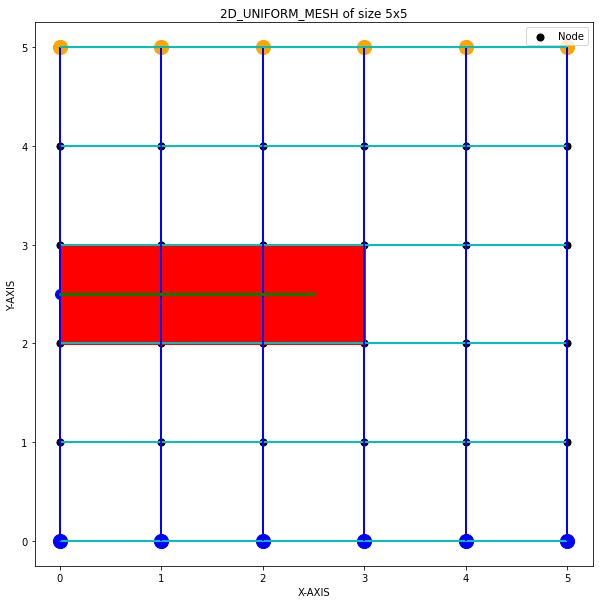
\includegraphics[scale=0.4]{enriched.png}
  \caption{Elements selected for the enrichment}
  \label{fig:1}
\end{figure}

\begin{figure}[h]
  \centering
  \includegraphics[scale=0.4]{Blend.png}
  \caption{Blended-elements}
  \label{fig:2}
\end{figure}

\begin{figure}[H]
  \centering
  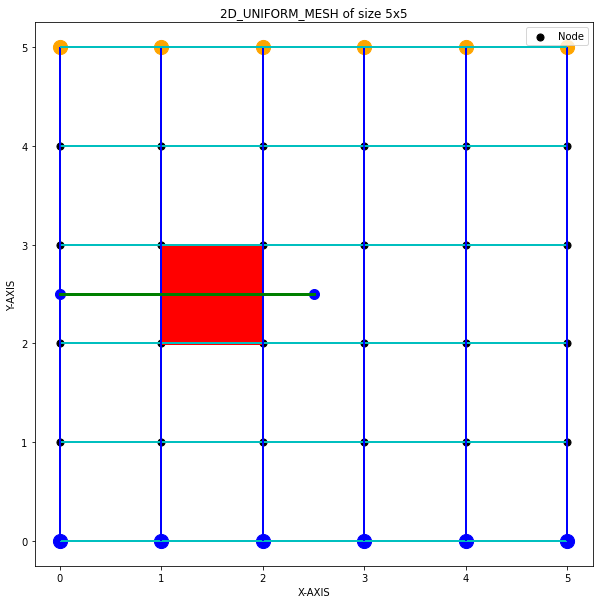
\includegraphics[scale=0.4]{pretip.png}
  \caption{Mixed enriched element}
  \label{fig:3}  
\end{figure}

\subsection{Heaviside step function}
The function usually takes the value of either +1 or 0 based on the function evaluated. the illustration is shown below see~\autoref{fig:4}. For an element completely cut by the crack, Heaviside function takes the value of +1, if the Gauss point is above the crack segment and -1 if the Gauss point is below the crack segment and will be 0 if it is lying on the crack segment. The step function is easy to calculate based on the sign of the $\Delta$ see.~\autoref{eq:6}. One of the easiest ways is the Orientation test\cite{ahmed2009extended}.\\

\begin{figure}[h]
    \centering
    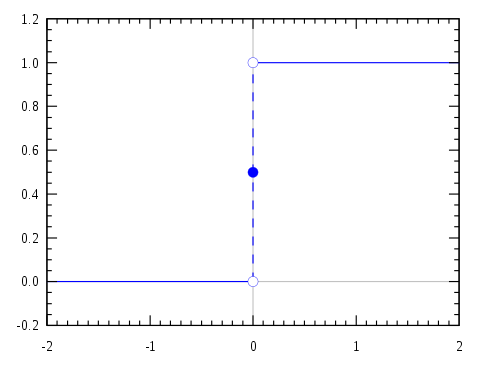
\includegraphics[scale =0.5]{Hside.png}
    \caption{Heaviside step-function} \cite{ahmed2009extended}
    \label{fig:4}
\end{figure}


\begin{align}\label{eq:6}
\hspace{5.25cm}H(x)\cite{ahmed2009extended} = 
\left\{
\begin{array}{ll}
+1 & sign| \Delta | > 0\\
\tab[0.1cm] 0 & sign| \Delta | = 0\\
-1 & sign| \Delta | < 0\\
\end{array}
\right.
\end{align}
$| \Delta |$, represents the determinant value of the matrix $\Delta$ which is calculated using orientation test

\subsection{Orientation test}
Orientation test determines whether the point under consideration is above or below the given line segments see~\autoref{fig:5}. The test is performed by evaluating a sign of the determinant. We formulate a triangle using 2 points from the crack segment and 1 query point and evaluating determinant will give the twice the area of a triangle. \\
It is obvious that, if the a triangle is formed above the crack segment, the sign of the determinant will be positive and should the triangle is formed below the crack segment, the sign of the determinant will be negative, and if the query point falls on the line, the determinant will have a zero value. Mathematically it can be expressed as see.~\autoref{eq:7}

\begin{figure}[h]%
    \centering
    \subfloat[\centering Query point "c" above]{{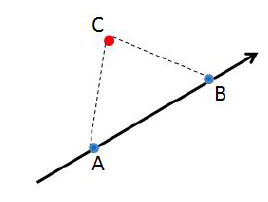
\includegraphics[width=7cm]{LHS.png}}}\hspace{1.5cm}
    \subfloat[\centering Query point "c" below]
    {{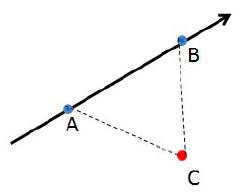
\includegraphics[width=7cm]{RHS.png}}}%
    \caption{Orientation test}\cite{ahmed2009extended}%
    \label{fig:5}
\end{figure}
\vspace{-0.25cm}
\begin{align}\label{eq:7}
\hspace{5.25cm}\Delta \cite{ahmed2009extended} =  
\begin{bmatrix}
a_x - c_x & a_y - c_y\\
b_x - c_x & b_y - c_y\\
\end{bmatrix}
\end{align}
In the above matrix see.~\autoref{eq:7}, 'a' and 'b' are the coordinates of the crack segment and 'c' is the coordinates of the point under query.
This methodology is applied for all the crack segments in a loop and the determinant value which has the least magnitude will be considered and the sign of that value is calculated.
\vsapce{-0.1cm}
\subsection{Heaviside Enrichment}
The nodes, that are enriched using Heaviside step function are called Heaviside enriched node. Each node that is Heaviside enriched will have 2 additional DOFs. Should all the nodes of the element are Heaviside enriched then the element will have a 16x16 element stiffness matrix. Below figure see~\autoref{fig:6} which element has been chosen for the heaviside enrichment.

\begin{figure}[h]
    \centering
    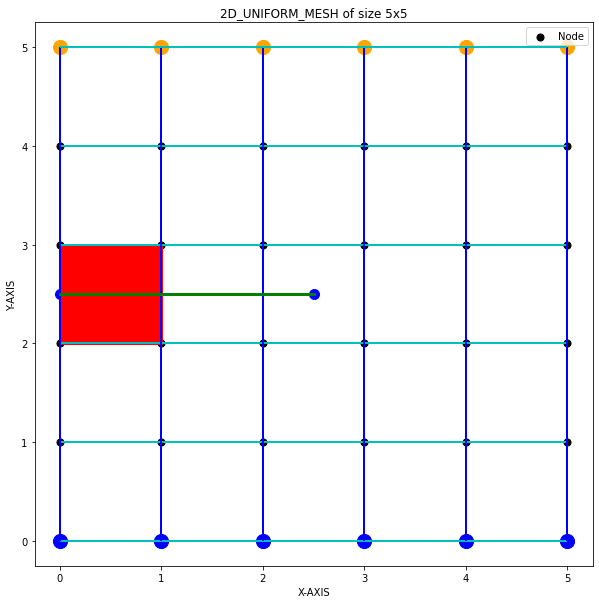
\includegraphics[scale = 0.30]{Heavy_enr.png}
    \caption{Heaviside enriched element}
    \label{fig:6}
\end{figure}

\subsection{Near-tip enrichment functions}
This is one of the extrinsic enrichment functions, which is used to enrich an element containing the crack tip. Branch functions are derived from the analytical solution using linear elastic fracture mechanics theory, and they are given as see.~\autoref{eq:8}. The element containing crack tip marked in red is shown in ~\autoref{fig:7}.

\begin{align}\label{eq:8}
\hspace{2.25cm}\beta_{\alpha}\cite{pandey2019new} = \left\{\beta_1, \beta_2, \beta_3, \beta_4 \right\} = \sqrt r \left[\cos\frac{\theta}{2}, \sin\frac{\theta}{2}, \cos\frac{\theta}{2} \sin{\theta}, \sin\frac{\theta}{2} \sin\theta \right]
\end{align}

\begin{figure}[h]
    \centering
    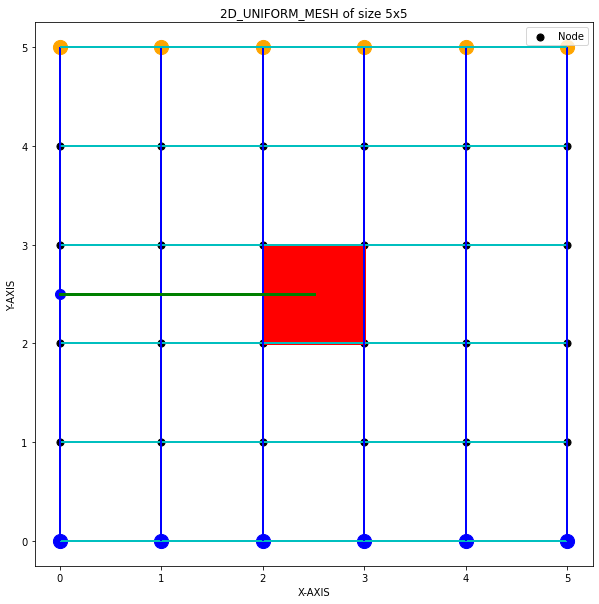
\includegraphics[scale =0.30]{Tip_enr.png}
    \caption{Tip enriched element}
    \label{fig:7}
\end{figure}

It should be mentioned here that $r$ and $\theta$ are in polar coordinates w.r.t crack tip.
$r$ is the distance measure from the point of the query to the crack tip see.~\autoref{eq:10} Ex:\space Node to crack tip, Gauss point to crack tip. It is vital to mention here that the distance measured, $r$, should be transformed from global coordinate system to crack tip coordinate system.

\begin{align}\label{eq:9}
\hspace{4.25cm}\begin{bmatrix} X_{ctcs} \\ Y_{ctcs}  \end{bmatrix}
=
\begin{bmatrix}
\cos\alpha & \sin\alpha\\
-\sin\alpha & \cos\alpha\\
\end{bmatrix}
*
\begin{bmatrix}
x_{global} - X_{tip}\\
y_{global} - Y_{tip}\\
\end{bmatrix}
\end{align}

\begin{align}\label{eq:10}
\hspace{4.25cm}r = \sqrt{X_{ctcs}^2 + Y_{ctcs}^2} \tab \theta = \arctan\left[\frac{Y_{ctcs}}{X_{ctcs}}\right]
\end{align}
$\alpha$ is the angle made by the crack w.r.t x-axis, $\theta$ should lie in the range of $0$ to $\pm \pi$, 'ctcs' is defined as crack tip coordinate system.\par
The nodes that are enriched using Near-tip enrichment functions are called tip enriched nodes/elements will have 8 additional DOFs these nodes are called Tip enriched nodes. The above figure properly illustrates the scenario. Suppose all the nodes of the element are Tip enriched then the element stiffness matrix will have a size 40x40 for the corresponding element. (8-classical DOFs, $\beta_1- 8 DOFs, \beta_2- 8 DOFs, \beta_3- 8 DOFs, \beta_4- 8 DOFs = 40 DOFs)$

\subsection{Derivatives of the near-tip enrichment functions}
The near-tip enrichment functions are represented in local polar coordinates and hence it has to be transformed to global Cartesian coordinate system. The derivatives of the enrichment functions with regard to global coordinates can be evaluated using the chain rule see.~\autoref{eq:11} and eq (12) \cite{mohammadi2008extended} 

\begin{align}\label{eq:11}
\hspace{5.25cm}\dv{F}{X} = \pdv{F}{r} \cdot \pdv{r}{X} + \pdv{F}{\theta} \cdot \pdv{\theta}{X} \\[7pt]
\dv{F}{Y} = \pdv{F}{r} \cdot \pdv{r}{Y} + \pdv{F}{\theta} \cdot \pdv{\theta}{Y}
\end{align}
\\
Derivatives of F$\alpha$ ($r$,$\theta$) with respect to the crack tip polar coordinates ($r$,$\theta$) is represented as see.~\autoref{eq:13} to see.~\autoref{eq:13}

\begin{align}\label{eq:13}
\hspace{3.25cm}F_{1,r} = \frac{1}{2\sqrt r} \sin\frac{\theta}{2}, \tab[1.25cm] F_{1,\theta} = \frac{\sqrt r}{2} \cos\frac{\theta}{2}
\end{align}

\begin{align}\label{eq:143}
\hspace{3.25cm}F_{2,r} = \frac{1}{2\sqrt r} \cos\frac{\theta}{2}, \tab[1.25cm] F_{2,\theta} = -\frac{\sqrt r}{2} \sin\frac{\theta}{2}
\end{align}

\begin{align}\label{eq:15}
\hspace{3.25cm}F_{3,r} = \frac{1}{2\sqrt r} \sin\frac{\theta}{2} \sin\theta, \tab[0.45cm] F_{3,\theta} = \sqrt r \left[\frac{1}{2}\cos\frac{\theta}{2} \sin\theta + \sin\frac{\theta}{2} \cos\theta \right]
\end{align}

\begin{align}\label{eq:16}
\hspace{3.25cm}F_{4,r} = \frac{1}{2\sqrt r} \cos\frac{\theta}{2} \sin\theta, \tab[0.45cm] F_{4,\theta} = \sqrt r \left[-\frac{1}{2}\sin\frac{\theta}{2} \sin\theta + \cos\frac{\theta}{2} \cos\theta \right]
\end{align}
and the derivatives of {$F_\alpha$} ($r$,$\theta$)\cite{mohammadi2008extended} with respect to the local crack coordinate system $(x', y')$ can then be defined as see.~\autoref{eq:17} to see.~\autoref{eq:20}

\begin{align}\label{eq:17}
\hspace{3.25cm}F_{1,x'} = -\frac{1}{2\sqrt r} \sin\frac{\theta}{2}, \tab[1.5cm] F_{1,y'} = \frac{1}{2\sqrt r} \cos\frac{\theta}{2}
\end{align}
\vspace{-1cm}
\begin{align}\label{eq:18}
\hspace{3.25cm}F_{2,x'} = \frac{1}{2\sqrt r} \cos\frac{\theta}{2}, \tab[1.75cm] F_{2,y'} = \frac{1}{2\sqrt r} \sin\frac{\theta}{2}
\end{align}

\begin{align}\label{eq:19}
\hspace{3.25cm}F_{3,x'} = -\frac{1}{2\sqrt r} \sin\frac{3\theta}{2} \sin\theta, \tab[0.45cm] F_{3,y'} = \frac{1}{2\sqrt r} \left[\sin\frac{\theta}{2} + \sin\frac{3\theta}{2} \cos\theta \right]
\end{align}

\begin{align}\label{eq:20}
\hspace{3.25cm}F_{4,x'} = -\frac{1}{2\sqrt r} \cos\frac{3\theta}{2} \sin\theta, \tab[0.45cm] F_{4,y'} = \frac{1}{2\sqrt r} \left[\cos\frac{\theta}{2} + \cos\frac{3\theta}{2} \cos\theta \right]
\end{align}

Finally, the derivatives of the asymptotic functions $F_{\alpha}$ \cite{mohammadi2008extended} in the global coordinate system are obtained by using the below \autoref{eq:21} to \autoref{eq:24}.
\begin{align}\label{eq:21}
\hspace{5.25cm}\pdv{r}{X} = \pdv{r}{x} \cdot \pdv{x}{X} + \pdv{r}{y} \cdot \pdv{y}{X}
\end{align}
\begin{align}\label{eq:22}
\hspace{5.25cm}\pdv{r}{Y} = \pdv{r}{x} \cdot \pdv{x}{Y} + \pdv{r}{y} \cdot \pdv{y}{X}
\end{align}
\begin{align}
\hspace{5.25cm}\pdv{\theta}{X} = \pdv{\theta}{x} \cdot \pdv{x}{X} + \pdv{\theta}{y} \cdot \pdv{y}{X}  
\end{align}
\begin{align}\label{eq:24}
\hspace{5.25cm}\pdv{\theta}{Y} = \pdv{\theta}{x} \cdot \pdv{x}{Y} + \pdv{\theta}{y} \cdot \pdv{y}{Y}   
\end{align}

where the derivatives of $r$ and $\theta$ w.r.t to x,y \cite{mohammadi2008extended} can be written as  \autoref{eq:25} and  \autoref{eq:26}
\begin{align}\label{eq:25}
\hspace{5.25cm}\pdv{r}{x} = \cos\theta \tab[0.45cm], \pdv{\theta}{x} = -\frac{\sin\theta}{r}
\end{align}
\begin{align}\label{eq:26}
\hspace{5.25cm}\pdv{r}{y} = \sin\theta,  \tab[0.45cm] \pdv{\theta}{y} = \frac{\cos\theta}{r}
\end{align}

\newline 
Using the transformation relationship between the global and crack tip coordinates we have ~\autoref{eq:27} and \autoref{eq:28}
\begin{align}\label{eq:27}
\hspace{5.25cm}\pdv{x}{X} = \cos\alpha,  \tab[0.45cm] \pdv{x}{Y} = \sin\alpha 
\end{align}
\begin{align}\label{eq:28}
\hspace{5.25cm}\pdv{y}{X} = -\sin\alpha, \tab[0.45cm] \pdv{y}{Y} = \cos\alpha
\end{align}

\section{ \large{Formulation of XFEM shape functions and B-matrix in the framework of Finite Element Method}}

Construction of XFEM shape function N matrix see.~\autoref{eq:30} and strain-displacement matrix B  see.~\autoref{eq:29} is straight forward. This section comprises of the detailed information regarding the generation of N and B matrices.

\begin{align}\label{eq:29}
\hspace{6.25cm}[B] = \begin{bmatrix}
B_{STD} & B_{enr}
\end{bmatrix}
\end{align}

\begin{align}\label{eq:30}
\hspace{6.25cm}[N] = 
\begin{bmatrix}
N_{STD} & N_{enr}
\end{bmatrix}   
\end{align}


\subsection{Shape functions}

\begin{figure}[h]
    \centering
    \includegraphics[scale = 1.8]{iso.png}
    \caption{Iso Parametric Element Mapping}\cite{sukumar2003modeling}
    \label{fig:8}
\end{figure}

The shape functions that are used in XFEM are same as the shape functions used in FEM. For a four noded iso-parametric quadrilateral element   see~\autoref{fig:8}, the standard FEM bi-linear shape functions  \cite{khoei2014extended}associated with each node are given as see.~\autoref{eq:31} to eq (34).

\begin{align}\label{eq:31}
\hspace{6.25cm}N1 = (1-\xi_1)(1-\xi_2) \\
\hspace{6.25cm}N2 = (1+\xi_1)(1-\xi_2) \\ 
\hspace{6.25cm}N1 = (1-\xi_1)(1-\xi_2) \\
\hspace{6.25cm}N2 = (1+\xi_1)(1-\xi_2)  
\end{align}
\vspace{-1.5cm}
The displacement approximation \cite{khoei2014extended} can then be written in the form of see.~\autoref{eq:35}
\begin{align}\label{eq:35}
\hspace{2.25cm}(X) = \large \begin{bmatrix}
N1 & 0 & N2 & 0 & N3 & 0 & N4 & 0\\
0 & N1 & 0 & N2 & 0 & N3 & 0 & N4\\
\end{bmatrix} \large
\cdot
\large \begin{bmatrix}
u_{x1}\\
u_{y1}\\
u_{x2}\\
u_{y2}\\
u_{x3}\\
u_{y3}\\
u_{x4}\\
u_{y4}\\
\end{bmatrix} \large
= N_{std}u
\end{align}

Where $u$ represents displacements of the given element. Each node has 2 DOFs hence the displacement matrix has a shape of 8x1. The standard FEM shape function matrix is given as see.~\autoref{eq:36}
\\
\begin{align}\label{eq:36}
\hspace{3cm}N_{STD} = \large \begin{bmatrix}
N1 & 0 & N2 & 0 & N3 & 0 & N4 & 0\\
0 & N1 & 0 & N2 & 0 & N3 & 0 & N4\\
\end{bmatrix} \large
\end{align}
\\
for a generic enrichment function, g(X), the enriched shape function matrix\cite{khoei2014extended} will be in the form of see.~\autoref{eq:37}
\begin{align}\label{eq:37}
\hspace{-1cm}N_{ENR} = \large \begin{bmatrix}[5]
(N_1g),x & 0 & (N_2g),x & 0 & (N_3g),x & 0 & (N_4g),x & 0 \\
0 & (N_1g),y & 0 & (N_2g),y & 0 &(N_3g),y & 0 & (N_4g),y
\end{bmatrix} \large
\end{align}

The shape functions are in local coordinate system and it should be transformed into global coordinate system. This is accomplished by using Jacobian matrix \cite{khoei2014extended} and the steps are as follows
\begin{itemize}
    \item Take the derivatives of the shape functions w.r.t $\xi_1$ and $\xi_2$ see.~\autoref{eq:38} to eq (41) and see.~\autoref{eq:42}
    \begin{align}\label{eq:38}
    \hspace{3.12cm}N_{1,\xi_1}= -\frac{1}{4}(1-\xi_2), \tab[0.25cm] N_{1,\xi_2}= - \frac{1}{4}(1-\xi_1)\\
    N_{2,\xi_1}=  \frac{1}{4}(1-\xi_2),  \tab[0.25cm] N_{2,\xi_2}= - \frac{1}{4}(1+\xi_1)\\
    N_{3,\xi_1}=  \frac{1}{4}(1+\xi_2),  \tab[0.25cm] N_{3,\xi_2}=  \frac{1}{4}(1+\xi_1)\\
    N_{4,\xi_1}= -\frac{1}{4}(1+\xi_2), \tab[0.25cm] N_{4,\xi_2}=  \frac{1}{4}(1-\xi_1)
    \end{align}
    
    \begin{align}\label{eq:42}
    \hspace{2cm}\pdv{[N]}{\xi} = \large \begin{bmatrix} 
    \dv{N_i} {\xi_1} \\[7pt]
    \dv{N_i} {\xi_2} \\
    \end{bmatrix} \large
    = 0.25*
    \begin{bmatrix}
    -(1-\xi_2) & 1-\xi_2 & 1+\xi_2 & -(1+\xi_2) \\
    -(1-\xi_1) & -(1+\xi_1) & 1+\xi_1 & 1 - \xi_1 \\
    \end{bmatrix}
    \end{align}
    \item Multiply the derivatives with the corresponding nodal coordinates see.~\autoref{eq:43} this gives the Jacobi matrix of 2x2.
    \begin{align}\label{eq:43}
    \hspace{6.25cm} J = \pdv{[N]}{\xi} \cdot (X^e)^T 
    \end{align}
    \item Take the inverse of the Jacobi matrix
    \item Multiply the inverse of the Jacobi matrix with the differentiated shape functions from step 1 generating a 2x4 matrix see.~\autoref{eq:44}.
    \begin{align}\label{eq:44}
    \hspace{6.25cm} \pdv{[N]}{x} = J^{-1} \cdot \pdv{[N]}{\xi} 
    \end{align}
    \item The elements in this matrix are arranged in a specified manner to get B-matrix see.~\autoref{eq:45}.  
    
\end{itemize}

\subsection{B-matrix}
This is also called as a Strain-Displacement matrix which gives a relation between strains and displacements see.~\autoref{eq:45}\cite{khoei2014extended}.
\begin{align}\label{eq:45}
\hspace{2.5cm} B_{std} = \begin{bmatrix}
N_{1,x} & 0 & N_{2,x} & 0 & N_{3,x} & 0 & N_{4,x} & 0 \\
0 & N_{1,y} & 0 & N_{2,y} & 0 & N_{3,y} & 0 & N_{4,y}\\
N_{1,y} & N_{1,x} & N_{2,y} & N_{2,x} & N_{3,y} & N_{3,x} & N_{4,y} & N_{4,x}
\end{bmatrix}
\end{align}
\\
Enriched B-matrix \cite{khoei2014extended} is given by see.~\autoref{eq:46}
\begin{align}\label{eq:46}
B_{enr} = \begin{bmatrix}
(N_1g),x & 0 & (N_2g),x & 0 & (N_3g),x & 0 & (N_4g),x & 0 \\
0 & (N_1g),y & 0 & (N_2g),y & 0 &(N_3g),y & 0 & (N_4g),y\\
(N_4g),y & (N_1g),x & (N_4g),y & (N_4g),x & (N_4g),y & (N_4g),x & (N_4g),y & (N_4g),x
\end{bmatrix}
\end{align}
$g(x)$ could be either Heaviside step function or Near Tip function. The below  \autoref{tab:Table1} gives the information on the additional degrees of freedom generated due to the enrichment
\begin{table}[h]
\begin{tabularx}{1\textwidth} { 
  | > {\centering\arraybackslash}X 
  | >{\centering\arraybackslash}X  
  | >{\centering\arraybackslash}X | }
  
 \hline
 \textbf {g(x)} & \textbf {Enrichment type} & \textbf {Degrees of freedom}\\
 \hline
 H(X) & Heaviside function or Heaviside step function & 2 DOFs per node\\
\hline
 $F^4 (r,\theta) $  & near-tip enrichment function & 8 DOFs per node\\
 \hline
\end{tabularx}
\caption{Table showing the additional DOFs for an enriched node}
\label{tab:Table1}
\end{table}

If the node is Heaviside enriched, the B-matrix\cite{khoei2014extended} is given by see.~\autoref{eq:47}
\begin{align}\label{eq:47}
\hspace{4cm} B_{Heavy} = \begin{bmatrix}
(N_i H(x))_x & 0\\
0 & (N_i H(x))_y\\
(N_i H(x))_y & (N_i H(x))_x
\end{bmatrix}
\: i=1,2,3,4
\end{align}
The derivative of Heaviside function is the Dirac delta function\cite{khoei2014extended}, that is see.~\autoref{eq:48}
\begin{align}\label{eq:48}
\hspace{5.5cm} (N_i H(x))_x = N_{i,x} H_{,x}(x) = \delta
\end{align}
If the node is tip enriched, the B-matrix \cite{khoei2014extended} is given by see.~\autoref{eq:49}
\begin{align}\label{eq:49}
\hspace{5cm} B_{tip} = \begin{bmatrix}
(N_i F_{\alpha})_,x & 0\\
0 & (N_i F_{\alpha})_,y\\
(N_i F_{\alpha})_,y & (N_i F_{\alpha})_,x\\
\end{bmatrix}
\: \alpha = 1,2,3,4
\end{align}
The derivative of near-tip enrichment function\cite{khoei2014extended} is given by see.~\autoref{eq:50}.
\begin{align}\label{eq:50}
\hspace{5.25cm}(N_i F_{\alpha})_,x = F_{\alpha} N_{i,x} + F_{\alpha,x} N_i\\
(N_i F_{\alpha})_,y = F_{\alpha} N_{i,y} + F_{\alpha,y} N_i
\end{align}
when $i=1, \alpha = 1,2,3,4$ \vspace{-0.5cm}
\begin{align}\label{eq:52}
\hspace{5.25cm}(N_1 F_1)_,x = F_1 N_{1,x} + F_{1,x} N_1\\[5pt]
(N_1 F_2)_,x = F_2 N_{1,x} + F_{2,x} N_1\\[5pt]
(N_1 F_3)_,x = F_3 N_{1,x} + F_{3,x} N_1\\[5pt]
(N_1 F_4)_,x = F_4 N_{1,x} + F_{4,x} N_1
\end{align}
Then the tip enriched B-matrix for 1 node is represented as see.~\autoref{eq:56},
\begin{align}\label{eq:56}
\hspace{-1cm}B_{tip} = \begin{bmatrix}
F_1 N_{1,x} + F_{1,x} N_1 & 0 & \dots  & F_4 N_{1,x} + F_{4,x} N_1 & 0\\
0 & F_1 N_{1,y} + F_{1,y} N_1 & \dots & 0 & F_4 N_{1,y} + F_{4,y} N_1\\
F_1 N_{1,y} + F_{1,y} N_1 & F_1 N_{1,x} + F_{1,x} & \dots & F_4 N_{1,y} + F_{4,y} N_1 & F_4 N_{1,x} + F_{4,x} N_1
\end{bmatrix}
\: \alpha = 1,2,3,4
\end{align}
\\
the same has to be implemented for the other 3 nodes if all 4 nodes in the element are tip enriched.

\subsection{Numerical Integration}

In the classical FEM, the standard shape functions are of the polynomial order and the Gauss integration rule can be used to evaluate the integral of stiffness matrix. However, in the X-FEM the enriched shape functions are obtained in terms of non-polynomial order. Moreover, the enrichment functions may not be smooth over an enriched element due to presence of the weak or strong discontinuity inside the element. Hence, the standard Gauss quadrature rule cannot be used if an element is crossed over by a crack, and necessary modifications are necessary for numerical integration over an enriched element\cite{khoei2014extended}. \par

The suggested approach is based on the increase of the
number of Gauss integration points\cite{khoei2014extended}, as shown in the below Figure \autoref{fig:9}, however, this  may also result in a substantial loss of accuracy. In order to overcome these difficulties, the enriched element will be divided into n-number of sub-polygons 
as shown in Figure, and the Gauss integration rule is performed over each sub-polygons. The sub-polygons do not produce additional DOFs\cite{khoei2014extended}. In the end all the K-matrices of the sub polygons will be summed up to get a K-matrix of the corresponding element.\par
Consider an element cut by an interface into two distinct parts, $\Omega+$ and $\Omega-$; the integration of stiffness matrix  over a domain (element) $\Omega$ can be performed using see.~\autoref{eq:57}

\begin{figure}[H]
    \centering
    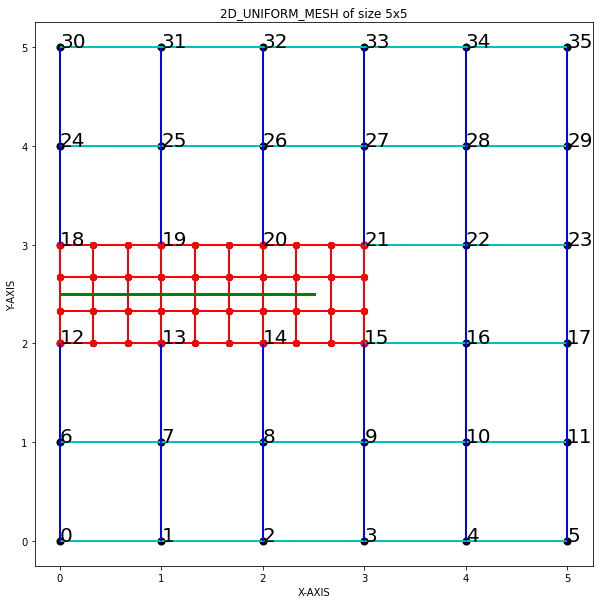
\includegraphics[scale =0.5]{Subdivision.png}
    \caption{9 Sub-polygons per element}
    \label{fig:9}
\end{figure}

$$\enspace K_{ij}^{\alpha\beta} = \int_{\Omega} B_{i(\xi_1,\xi_2)}^T*D*B_{j(\xi_1,\xi_2)}*| J | d\xi_1d\xi_2$$\vspace{0.1cm}
$$ = \int_{\Omega+} B_{i(\xi_1,\xi_2)}^T*D*B_{j(\xi_1,\xi_2)}*| J | d\xi_1d\xi_2 + \int_{\Omega-} B_{i(\xi_1,\xi_2)}^T*D*B_{j(\xi_1,\xi_2)}*| J | d\xi_1d\xi_2 $$\vspace{0.1cm}
\begin{align}\label{eq:57}
\hspace{-1.5cm}= \sum_{l=1}^{\mathscr{N}^{SUB+}} \left(\sum_{k=1}^{\mathscr{N}^{GP+}} B_{i(\xi_{1k},\xi_{2k})}^T*D*B_{j(\xi_{1k},\xi_{2k})}*w_k \right)_l  + \sum_{l=1}^{\mathscr{N}^{SUB-}} \left(\sum_{k=1}^{\mathscr{N}^{GP-}} B_{i(\xi_{1k},\xi_{2k})}^T*D*B_{j(\xi_{1k},\xi_{2k})}* w_k \right)_l
\end{align}
where in ${\mathscr{N}^{SUB+}}$ and ${\mathscr{N}^{SUB-}}$ are the number of sub-polygons in $\Omega+$ and $\Omega-$, and ${\mathscr{N}^{GP+}}$ and ${\mathscr{N}^{GP-}}$ are the number of Gauss points at each sub-polygon in $\Omega+$ and $\Omega-$, respectively.In this relation, $w_k$ is the weight of quadrature point. Therefore, Gauss quadrature can be employed, which allows integration of polynomials up to a certain order in the given element. 

\subsection{Element connectivity matrix}
The matrix which is used to assemble all the element stiffness matrix. The matrix consists of only 0s and 1s. The size of the connectivity matrix is decided based on the number of DOFs available in the geometry. The columns of the matrix is the maximum DOFs available in the geometry and the rows of the matrix is the maximum DOFs available in the single element. As mentioned in the previous section, the additional DOFs will be placed in the last columns and rows after allotting rows and columns for normal DOFs. The equation for generating an assignment matrix is given by  see.~\autoref{eq:58}

\begin{align}\label{eq:58}
A_{matrix} = [Max\hspace{0.1cm} DOFs\hspace{0.1cm} availabe\hspace{0.1cm} in \hspace{0.1cm} element]\hspace{0.1cm} *\hspace{0.1cm} [Max\hspace{0.1cm} DOFs \hspace{0.1cm}availabe\hspace{0.1cm} in\hspace{0.1cm} the\hspace{0.1cm} geometry]
\end{align}

\subsection{ {Element stiffness matrix}}
The element stiffness matrix for classical element is given by see.~\autoref{eq:59}
and see.~\autoref{eq:60}\cite{khoei2014extended}

\begin{align}\label{eq:59}
\hspace{5cm}K = \int_{-1}^{1} \int_{-1}^{1} B_{\xi_1, \xi_2}^T*D*B_{\xi_1, \xi_2}*| J | d\xi_1d\xi_2 
\end{align}
The BVP is solved using
\begin{align}\label{eq:60}
\hspace{6.25cm}[K][u] = [F] 
\end{align}\vspace{-1cm}
\\
Wherein \newline
\tab[1cm] K = $K_{global}$, is called the global stiffness matrix\newline
\tab[1cm] u = Displacement matrix\newline
\tab[1cm] F = Force vector

\subsection{Nodal Displacements}
After solving BVP, a 1D displacement vector is obtained. This vector contains both classical and enriched displacements. It should be noted that if there a node is enriched, then displacement of that node will be summed with the enriched displacements and multiplied with the enrichment function value. Using the displacement approximation equation, corresponding nodal displacements are calculated. The relation handles both classical and enriched displacements  see.~\autoref{eq:61}.

\begin{align}\label{eq:61}
\hspace{3cm}u(x) = \sum_{i=1}^n N_i(x)u_i + \sum_{j^{heavy}=1}^P N_j(x)[\psi(x)] a_j + \sum_{k^{tip}=1}^4 N_k(x)[\beta_{\alpha}(x)] b_{k^\alpha} 
\end{align}

The displacements that are calculated using XFEM should be treated the same way as the stresses. But before transforming, one should calculate the gradient of the XFEM displacements \cite{ahmed2009extended} and it is given by  see.~\autoref{eq:62}
\vspace{-1.2cm}
\begin{align}\label{eq:62}
\hspace{-1cm}\begin{bmatrix}
u_{x(XFEM)} & u_{y(XFEM)}\\
v_{x(XFEM)} & v_{y(XFEM)}\\
\end{bmatrix}
=
B_{std} = \begin{bmatrix}
N_{1,x} & 0 & N_{2,x} & 0 & N_{3,x} & 0 & N_{4,x} & 0 \\
0 & N_{1,y} & 0 & N_{2,y} & 0 & N_{3,y} & 0 & N_{4,y}\\
\end{bmatrix}
*
\large \begin{bmatrix}
u_{x1}\\
u_{y1}\\
u_{x2}\\
u_{y2}\\
u_{x3}\\
u_{y3}\\
u_{x4}\\
u_{y4}\\
\end{bmatrix} \large
\end{align}

Transformation of displacement gradients to crack tip coordinate system  see.~\autoref{eq:63}
\begin{align}\label{eq:63}
\hspace{0.5cm}\begin{bmatrix}
U_{X (CTCS)} & U_{Y (CTCS)}\\
V_{X (CTCS)} & V_{Y (CTCS)}\\
\end{bmatrix}
=
\begin{bmatrix}
\cos\alpha & \sin\alpha\\
-\sin\alpha & \cos\alpha\\
\end{bmatrix}
*
\begin{bmatrix}
u_{x (XFEM)} & u_{y (XFEM)}\\
v_{x (XFEM)} & v_{y (XFEM)}\\
\end{bmatrix}
*
\begin{bmatrix}
\cos\alpha & -\sin\alpha\\
\sin\alpha & \cos\alpha\\
\end{bmatrix}
\end{align}

\subsection{Calculation of Stresses and Strains}
After the computation of displacements, strains must be calculated using strain-displacement matrix (B-matrix) and it is given by see.~\autoref{eq:64} and see.~\autoref{eq:65}

\begin{align}\label{eq:64}
\hspace{6.25cm}\epsilon = [B][u]
\end{align}

\begin{align}\label{eq:65}
\hspace{2cm}\begin{bmatrix}
\epsilon_x\\
\epsilon_y\\
\gamma_{xy}\\
\end{bmatrix}
=
\begin{bmatrix}
N_{1,x} & 0 & N_{2,x} & 0 & N_{3,x} & 0 & N_{4,x} & 0 \\
0 & N_{1,y} & 0 & N_{2,y} & 0 & N_{3,y} & 0 & N_{4,y}\\
N_{1,y} & N_{1,x} & N_{2,y} & N_{2,x} & N_{3,y} & N_{3,x} & N_{4,y} & N_{4,x}
\end{bmatrix}
*
\large \begin{bmatrix}
u_{x1}\\
u_{y1}\\
u_{x2}\\
u_{y2}\\
u_{x3}\\
u_{y3}\\
u_{x4}\\
u_{y4}\\
\end{bmatrix} \large
\end{align}
wherein $\epsilon$ is the strain and B is B-matrix and u is the nodal displacements.
\newline
Stresses are calculated using the see.~\autoref{eq:66} and plane stress relation see.~\autoref{eq:67}
\begin{align}\label{eq:66}
\hspace{6.25cm}\sigma = [D][\epsilon]
\end{align}

\begin{align}\label{eq:67}
\hspace{5cm}\begin{bmatrix}
\sigma_x\\
\sigma_y\\
\sigma_{xy}\\
\end{bmatrix}
=
\frac{E}{1-\nu^2}
\begin{bmatrix}
1 & \nu & 0\\
\nu & 1 & 0\\
0 & 0 & \frac{1-\nu}{2}\\
\end{bmatrix}
*
\begin{bmatrix}
\epsilon_x\\
\epsilon_y\\
\gamma_{xy}\\
\end{bmatrix}
\end{align}

The stresses, that are calculated using XFEM should be transformed from global coordinate system to crack tip coordinate system using appropriate rotation matrix \cite{ahmed2009extended} and the equation is given by see.~\autoref{eq:68} 
\begin{align}\label{eq:68}
\hspace{0cm}\begin{bmatrix}
\sigma_{XX (CTCS)} & \sigma_{XY (CTCS)}\\
\sigma_{XY (CTCS)} & \sigma_{YY (CTCS)}\\
\end{bmatrix}
=e
\begin{bmatrix}
\cos\alpha & \sin\alpha\\
-\sin\alpha & \cos\alpha\\
\end{bmatrix}
*
\begin{bmatrix}
\sigma_{xx (XFEM)} & \sigma_{xy (XFEM)}\\
\sigma_{yx (XFEM)} & \sigma_{yy (XFEM)}\\
\end{bmatrix}
*
\begin{bmatrix}
\cos\alpha & -\sin\alpha\\
\sin\alpha & \cos\alpha\\
\end{bmatrix}
\end{align}
%===============================================================================
\section{\large{Linear Elastic Fracture mechanics}}
\subsection{Introduction}

Strength of the materials were computed in the past based on two possible theories [Griffith 1921]. A material is said to fracture if maximum tensile stress or maximum extension in a body exceeds a certain threshold value\cite{kuna2013finite}. Hence the strength of the material is basically considered to be an intrinsic property. \\
One of earliest recorded incidents of brittle fracture failure was the Montrose bridges 1830 [Erdogan 2000]. There have been many incidents due to fracture failure after that e.g the event of Tay Rail Bridge failure in 1879 \cite{kuna2013finite}. These incidents led the scientists and engineers to exploit the Fracture mechanics domain. 
It is said that Griffith’s and Irwin’s work has led the foundations for a new engineering branch “Engineering Fracture Mechanics” to flourish, and soon after that Fracture mechanics evolved as an important branch in the engineering realm. 
A very good review on fracture mechanics can be found in Erdogan [2000]. More details on engineering fracture mechanics can also be found in \cite{kuna2013finite}

\subsection{Modes of Failure}
Failure is defined as the rupture of the sample under the applied load. There are three modes of failure, namely Mode I, Mode II, and Mode III \cite{kuna2013finite}.
\begin{itemize}
    \item Mode I: is the opening type \autoref{fig:10} wherein a tensile load is applied normal to the crack surfaces and crack opens perpendicular to the crack plane i.e. the crack propagation angle is 0.
    \item Mode II: A shear load is applied parallel to the crack surfaces \autoref{fig:11} and the crack is allowed to propagate. The crack propagation angle varies from +70 degrees to -70 degrees. The crack faces are found to be sliding in the direction of applied load.
    \item Mode III: a shear stress is applied perpendicular to the plane of the crack \autoref{fig:12}. This is also called as Out-of-plane tearing mode.
\end{itemize}
The three modes of failures are shown schematically in the below figures.

\begin{figure}[H]
  \begin{minipage}[b]{0.4\textwidth}
    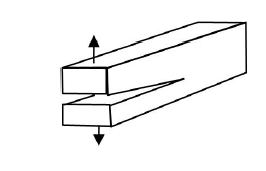
\includegraphics[scale = 0.8]{M1.png}
    \caption{{Mode-I Type failure \cite{kuna2013finite}}}
    \label{fig:10}
  \end{minipage}
  \hspace{2cm}
  \begin{minipage}[b]{0.4\textwidth}
    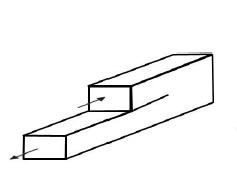
\includegraphics[scale = 0.8]{M2.png}
    \caption{{Mode-II Type failure \cite{kuna2013finite}}}
    \label{fig:11}
  \end{minipage}
\end{figure}

\begin{figure}[h]
    \centering
    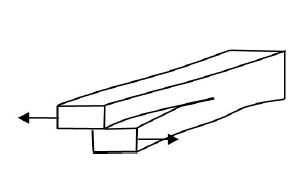
\includegraphics[scale = 0.8]{M3.png}
    \caption{{Mode-III Type failure \cite{kuna2013finite}}}
    \label{fig:12}
\end{figure}

\section{ \large{Displacement and Stress Fields at the Crack Tip Area}}

The importance of stress singularity at the crack tip area was presented by Westergaard (1939) and Williams (1957) by evaluation of the displacement and stress fields around the crack tip area \autoref{fig:13}. Williams (1957) used the Airy stress function to capture the singularity at the crack tip area using a polar coordinate system \cite{khoei2014extended} $(r, \theta)$ as given in see.~\autoref{eq:69}

\begin{align}\label{eq:69}
\hspace{2cm}\Phi = r^{\lambda+1} (c_1 \sin(\lambda+1)\hat{\theta} + c_2 \cos(\lambda+1)\hat{\theta} + c_3 \sin(\lambda-1)\hat{\theta} + c_4 \sin(\lambda-1)\hat{\theta})
\end{align}

wherein $c_i$ are the coefficients and $\hat{\theta}$ is depicted in the below Figure
\begin{figure}[h]
    \centering
    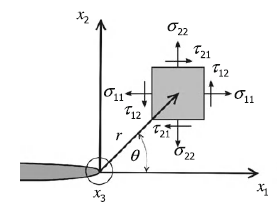
\includegraphics[scale = 1]{stress.PNG}
    \caption{{Stresses at the crack tip in Cartesian coordinates     \cite{kuna2013finite}}}
    \label{fig:13}
    \centering
\end{figure}
%------------------------------------------------------------------------------------
\subsection{{Auxiliary displacements for mode-I}}
Substituting the Airy stress function EQUATION in the equilibrium equation of the system, that is, $\bigtriangledown^2 \bigtriangledown^2\Phi = 0$ \cite{khoei2014extended}
in the absence of body forces, applying the traction-free boundary conditions at the crack faces. It should be noted here that the displacement field is a function of crack tip polar coordinate system and we are required to find the spatial derivatives according to the local crack tip Cartesian coordinate system \cite{nagashima2003stress}. This will be evaluated as see.~\autoref{eq:70} to see.~\autoref{eq:72}

\begin{align}\label{eq:70}
\hspace{3.5cm}U_x = \frac{K_I (1+\nu)}{E} \sqrt{\frac{r}{2\pi}} \cos\frac{\theta}{2} \left[k-1+2\sin^2\frac{\theta}{2} \right]\\[8pt]
U_y = \frac{K_I (1+\nu)}{E} \sqrt{\frac{r}{2\pi}} \sin\frac{\theta}{2} \left[k+1-2\cos^2\frac{\theta}{2} \right]
\end{align}
\vspace{-1.5cm}
\begin{align}\label{eq:72}
\hspace{3.5cm}U_z = 0
\end{align}

Derivatives of the displacement $U_x$ and $U_y$ w.r.t to $x$ and $y$ \cite{nagashima2003stress} is given in see.~\autoref{eq:73} to eq (76)

\begin{align}\label{eq:73}
\hspace{4.5cm}\dv{U_x}{X} = \dv{U_x}{r}*\dv{r}{X} + \dv{U_x}{\theta}*\dv{\theta}{X}\\[8pt]
\dv{U_x}{Y} = \dv{U_x}{r}*\dv{r}{Y} + \dv{U_x}{\theta}*\dv{\theta}{Y} \\[8pt]
\dv{U_y}{X} = \dv{U_y}{r}*\dv{r}{X} + \dv{U_y}{\theta}*\dv{\theta}{X} \\[8pt]
\dv{U_y}{Y} = \dv{U_y}{r}*\dv{r}{Y} + \dv{U_y}{\theta}*\dv{\theta}{Y}
\end{align}
\\
Derivatives of the displacement $U_x$ and $U_y$ w.r.t to $r$ and $\theta$ \cite{nagashima2003stress}is given by see.~\autoref{eq:77} to see.~\autoref{eq:80} 
\begin{align}\label{eq:77}
\hspace{4.5cm}\dv{U_x}{r} = \frac{K_I(1+\nu)}{2D} \frac{1}{\sqrt{2\pi r}} \cos\frac{\theta}{2} (k-\cos\theta)
\end{align}

\begin{align}\label{eq:78}
\hspace{4.5cm}\dv{U_x}{\theta} = \frac{K_I(1+\nu)}{D} \sqrt{\frac{r}{2\pi}} \left[-0.5\sin\frac{\theta}{2} (k-\cos\theta) + \sin\theta \cos\frac{\theta}{2} \right]
\end{align}

\begin{align}\label{eq:79}
\hspace{4.5cm}\dv{U_y}{r} = \frac{K_I(1+\nu)}{2D} \frac{1}{\sqrt{2\pi r}} \sin\frac{\theta}{2} (k-\cos\theta)
\end{align}

\begin{align}\label{eq:80}
\hspace{4.5cm}\dv{U_x}{\theta} = \frac{K_I(1+\nu)}{D} \sqrt{\frac{r}{2\pi}} \left[0.5\cos\frac{\theta}{2} (k-\cos\theta) + \sin\theta \sin\frac{\theta}{2} \right]
\end{align}

Derivatives $r$ and $\theta$ w.r.t to $x$ and $y$ \cite{khoei2014extended} is given by see.~\autoref{eq:81} and eq(82)
\begin{align}\label{eq:81}
\hspace{4.5cm}\dv{r}{X} = \cos\theta, \tab[1cm] \dv{r}{Y} = \sin\theta \\[8pt]
\dv{\theta}{X} = -\sin\frac{\theta}{r}, \tab[1cm] \dv{\theta}{Y} = \cos\frac{\theta}{r}
\end{align}
%-------------------------------------------------------------------------------

\subsection{Auxiliary stresses for mode-I}
The Auxiliary stresses in case of mode I is given by \autoref{eq:83} to \autoref{eq:86} \cite{khoei2014extended}

\begin{align}\label{eq:83}
\hspace{4.5cm}\sigma_{x} = \frac{K_I}{\sqrt{2\pi r}} \cos\frac{\theta}{2} \left[1-\sin\frac{\theta}{2} \sin\frac{3\theta}{2}\right]\\[8pt]
\sigma_{y} = \frac{K_I}{\sqrt{2\pi r}} \cos\frac{\theta}{2} \left[1+\sin\frac{\theta}{2} \sin\frac{3\theta}{2}\right]\\[8pt]
\tau_{xy} = \frac{K_I}{\sqrt{2\pi r}} \sin\frac{\theta}{2} \cos\frac{\theta}{2} \cos\frac{3\theta}{2}
\end{align}

\begin{align}\label{eq:86}\hspace{4.5cm}
\sigma_{z} = 
\left\{
\begin{array}{ll}
\nu(\sigma_x + \sigma_y) & \mbox{Plane strain}\\
\tab[0.75cm] 0 & \mbox{Plane stress}\\
\end{array}
\right.
\end{align}

%---------------------------------------------------------------------------------------------
\subsection{Auxiliary displacements for mode-II}
The displacements for mode-II is given by \autoref{eq:87} to \autoref{eq:89} \cite{khoei2014extended}

\begin{align}\label{eq:87}\hspace{4.5cm}
U_x = \frac{K_{II}(1+\nu)}{E} \sqrt{\frac{r}{2\pi}} \sin\frac{\theta}{2} \left[k+1+2\cos^2\frac{\theta}{2} \right]
\end{align}

\begin{align}\label{eq:88}\hspace{4.5cm}
U_y = \frac{K_{II}(1+\nu)}{E} \sqrt{\frac{r}{2\pi}} \cos\frac{\theta}{2} \left[k-1-2\sin^2\frac{\theta}{2} \right]
\end{align}

\begin{align}\label{eq:89}
\hspace{4.5cm}U_z = 0
\end{align}

Derivatives of the displacement $U_x$ and $U_y$ w.r.t to $r$ and $\theta$ \cite{nagashima2003stress} is given in \autoref{eq:90} to \autoref{eq:93}

\begin{align}\label{eq:90}\hspace{4.5cm}
\dv{U_x}{r} = \frac{K_{II}(1+\nu)}{2D} \frac{1}{\sqrt{2\pi r}} \cos\frac{\theta}{2} (k+2+\cos\theta)
\end{align}

\begin{align}\label{eq:91}\hspace{4.5cm}
\dv{U_x}{\theta} = \frac{K_{II}(1+\nu)}{D} \sqrt{\frac{r}{2\pi}} \left[0.5\cos\frac{\theta}{2} (k+2+\cos\theta) - \sin\theta \sin\frac{\theta}{2} \right]
\end{align}

\begin{align}\label{eq:92}\hspace{4.5cm}
\dv{U_y}{r} = \frac{K_{II}(1+\nu)}{2D} \frac{1}{\sqrt{2\pi r}} \cos\frac{\theta}{2} (k-2+\cos\theta)
\end{align}

\begin{align}\label{eq:93}\hspace{3.5cm}
\dv{U_x}{\theta} = -\frac{K_{II}(1+\nu)}{D} \sqrt{\frac{r}{2\pi}} \left[-0.5\sin\frac{\theta}{2} (k-2+\cos\theta) +- \sin\theta \cos\frac{\theta}{2} \right]
\end{align}

\subsection{Auxiliary stresses for mode-II}
The Auxiliary stresses in case of mode II is given by \autoref{eq:94} to \autoref{eq:97} \cite{khoei2014extended}

\begin{align}\label{eq:94}\hspace{4.5cm}
\sigma_{x}\cite{ahmed2009extended} = -\frac{K_{II}}{\sqrt{2\pi r}} \sin\frac{\theta}{2} \left[2+\cos\frac{\theta}{2} \cos\frac{3\theta}{2}\right]
\end{align}

\begin{align}\label{eq:95}\hspace{4.5cm}
\sigma_{y}\cite{ahmed2009extended} = \frac{K_{II}}{\sqrt{2\pi r}} \sin\frac{\theta}{2} \cos\frac{\theta}{2} \cos\frac{3\theta}{2}
\end{align}

\begin{align}\label{eq:96}\hspace{4.5cm}
\tau_{xy}\cite{ahmed2009extended} = \frac{K_{II}}{\sqrt{2\pi r}} \cos\frac{\theta}{2} \left[1-\sin\frac{\theta}{2} \sin\frac{3\theta}{2}\right]
\end{align}

\begin{align}\label{eq:97}\hspace{4.5cm}
\sigma_{z}\cite{ahmed2009extended} = 
\left\{
\begin{array}{ll}
\nu(\sigma_x + \sigma_y) & \mbox{Plane strain}\\
\tab[0.75cm] 0 & \mbox{Plane stress}\\
\end{array}
\right.
\end{align}

Wherein "k" in see.~\autoref{eq:90} is called Kolosov constant and it is defined as $k=(3-\nu)/(1+\nu)$ for plane stress and $k=3-4\nu$ for plane strain problems and $\nu$ is the Poisson ratio. D is Young's modulus.
\\
In the above relations see.~\autoref{eq:90} and see.~\autoref{eq:94}, $K_{I}$, and $K_{II}$ are the SIFs for mode-I and mode-II respectively and they are given by \autoref{eq:98} and \autoref{eq:99}.

\begin{align}\label{eq:98}\hspace{4.5cm}
K_I = \sigma_y \sqrt{2*\pi r} \tab[0.25cm] MPa\sqrt{m}
\end{align}

\begin{align}\label{eq:99}\hspace{4.5cm}
K_{II} = \sigma_{xy} \sqrt{2*\pi r} \tab[0.25cm] MPa\sqrt{m}    
\end{align}

wherein
\\
\tab[1cm] $\mathbold{\sigma_{x}}$ = Tensile Stress in MPa
\\
\tab[1cm] $\mathbold{\sigma_{xy}}$ = Shear Stress in MPa
\\
\tab[1cm] \textbf{r} = crack length in m

\section{\large{Stress Intensity Factors}}

In the linear elastic fracture mechanics (LEFM), the stress, strain, and displacement fields can be determined by employing the concept of the SIFs near the crack tip region. It is therefore important to accurately evaluate the SIFs for the FE analysis of LEFM.\\

There are many computational algorithms available to evaluate the SIFs. The approaches can be categorized into two groups; the “direct” approach and the “energy” approach. The direct approach relates the SIFs with the FEM results directly, while the energy approach is based on the computation of energy release rate. In general, the energy approaches are more accurate than the direct procedures. However, the direct approaches are more popular and are usually used to verify the results of energy approaches, since their expressions are simple. The most popular energy approach is the J-integral technique\cite{khoei2014extended}. In the following section the J-integral method is discussed in detail

\subsection{J-integral}
In Fracture mechanics computations, SIFs are the most important fracture parameters used for the determination of mixed-mode near tip stress, strain, and displacement fields. In order to evaluate the SIFs, the area J–integral is defined in relation \eqref{eq:100} and see.~\autoref{eq:101}, which can be computed over an area of the FE mesh refer to the figure below \autoref{fig:14}. In XFEM modeling, the area for the integration is calculated by assuming a virtual circle with a specific radius around the crack tip, and the integration is performed over the elements that lie inside the circle \cite{kuna2013finite}, as shown in Figure 7.16. 
\begin{figure}[h]
    \centering
    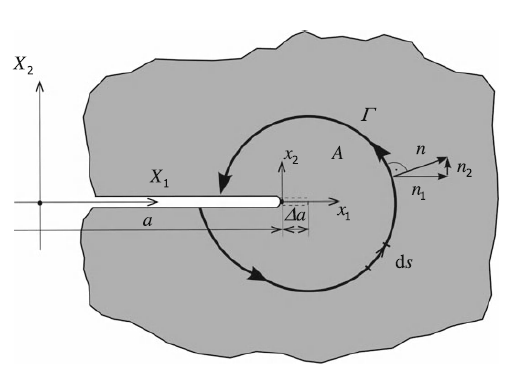
\includegraphics[scale = 1]{J_int.PNG}
    \caption{{Elements inside the area are integrated\cite{kuna2013finite}}}
    \label{fig:14}

\end{figure}    
    
Basically, J-integral is calculated by adding the integrals computed for a sample without a crack (Auxiliary state / state (2)) and the same sample with crack (current configuration/ state(1)). For this purpose, BVP is solved using XFEM to obtain to obtain the displacement, strain, and stress fields of state (1) that is, $u_i^{(1)}$, $\epsilon_{ij}^{(1)}$, and $\sigma_{ij}^{(1)}$ and these values are then transferred from the global to local crack tip coordinate system $(x_1, x_2)$ by using an appropriate transformation.

\begin{align}\label{eq:100}\hspace{4.5cm}
J = \int_A \left(\sigma_{ij} \pdv{u_i}{x_1} - \mathscr{W}\delta_{ij}\right) \pdv{q}{x_j}dA
\end{align}

\begin{align}\label{eq:101}\hspace{4.5cm}
I^{(1,2)} = \int_A \left(- \mathscr{W}^{(1,2)}\delta_{1j} + \sigma_{ij}^{(1)} \pdv{u_i^{(2)}}{x_1} + \sigma_{ij}^{(2)} \pdv{u_i^{(1)}}{x_1}\right) \pdv{q}{x_j}dA
\end{align}

Wherein $\mathscr{W}^{(1,2)}$ is the interaction strain energy \cite{kuna2013finite} defined by see.~\autoref{eq:102}

\begin{align}\label{eq:102}\hspace{4.5cm}
\mathscr{W}^{(1,2)} = \sigma_{ij}^{(1)} \epsilon_{ij}^{(2)} = \sigma_{ij}^{(2)} \epsilon_{ij}^{(1)}
\end{align}

The super scripts $(2)$, and $(1)$ implicates auxiliary state(material without crack) and current state(after the introduction of the crack) respectively.
The distribution of weighting function q in the above relation can be obtained for an element using the standard FE interpolation \cite{kuna2013finite} as see.~\autoref{eq:103}

\begin{align}\label{eq:103}\hspace{4.5cm}
q = \sum_{I=1}^{\mathscr{N}^{elem}} N_I(x)q_I
\end{align}

where ${\mathscr{N}^{elem}}$ is the number of nodes of an element and $q_I$ are the nodal values of q. The derivation of weighting function can be obtained as see.~\autoref{eq:104}

\begin{align}\label{eq:104}\hspace{4.5cm}
\pdv{q}{x} = \sum_{I=1}^{\mathscr{N}^{elem}} \pdv{N_I}{x}q_I
\end{align}

After calculating the derivative of the weight function see.~\autoref{eq:104}, $\pdv{q}{x}$ is converted to local crack tip coordinate system using appropriate transformation see.~\autoref{eq:105}.

\begin{align}\label{eq:105}\hspace{4.5cm}
\left[\pdv{q}{X}\right] = [R] * \left[\pdv{q}{x}\right] 
\end{align}

where R in the above equation is called rotation matrix and it is defined as see.~\autoref{eq:106}

\begin{align}\label{eq:106}\hspace{4.5cm}
\large \begin{bmatrix} 
\pdv{q} {X} \\[7pt]
\pdv{q} {Y} \\
\end{bmatrix} \large
=
\begin{bmatrix}
\cos\alpha & \sin\alpha\\
-\sin\alpha & \cos\alpha\\
\end{bmatrix}
*
\large \begin{bmatrix} 
\pdv{q} {x} \\[7pt]
\pdv{q} {y} \\
\end{bmatrix} \large
\end{align}

\hspace{-0.5cm}{\color{black} \rule{\linewidth}{0.05cm}}
	{\scshape Function Body of the Interaction integral}\\
{\color{black} \rule{\linewidth}{0.05cm}}
{\fontfamily{qcr}\selectfont
def Interaction{\_}integral(Nodes, displacements, stress, strains, set4Gauss, c{\_}2, GaussPoint{\_}1to4, l{\_}x, l{\_}y, D{\_}plane{\_}stress, alpha, CL, A, force, D, scale, \\
increment)\\
    The function computes the SIFs using domain integral technique\\
    Parameters:\\
    ---------------------\\
    Nodes : List of 4 nodal coordinates\\
    displacements : List of Element displacements (8 per element)\\
    stress : List of 3 stress values\\
    strains: List of 3 strain values\\
    set4Gauss: Gauss coordinates in global system\\
    c{\_}2: Crack tip coordinates\\
    GaussPoint{\_}1to4 : 4 Gauss coordinates \\
    l{\_}x, l{\_}y: Length of Element along x and y axes\\
    D{\_}plane{\_}stress: Plane stress relation\\
    alpha: Angle made by crack tip w.r.t x-axis\\
    CL, A: Crack length, Geometry length along X\\
    force: Applied force\\
    D: Young's modulus\\
    scale: Scaling factor for the domain\\
    Returns: KI, KII}
    
\subsection{The Maximum Circumferential Tensile Stress Criterion}
The maximum circumferential tensile stress theory was first presented by Erdogan and Sih (1963) based on the state of stress near the crack tip. Based on this theory, the crack propagates at the crack tip in a radial direction on the plane perpendicular to the direction of maximum tension \cite{khoei2014extended}.\\
In the current case, the hoop stress reaches its maximum value on the plane of zero shear stress. It is assumed that the size of plastic zone at the crack tip is negligible, the singular term solutions of stress at the crack tip can be used to determine the crack propagation angle, where the shear stress becomes zero \cite{khoei2014extended}.
\\
The critical angle of crack propagation $\theta_c$ can be determined using \autoref{eq:107}
\begin{equation}\label{eq:107}\hspace{4.5cm}
\frac{1}{\sqrt{2 \pi r}} \cos \frac{\theta}{2}\left[\frac{1}{2} K_{I} \sin \theta+\frac{1}{2} K_{I I}(3 \cos \theta-1)\right]=0
\end{equation}

The solution of this equation results in the crack propagation angle θc that can be expressed using the angle between the line of crack and the crack growth direction, with the positive value defined in an anti-clockwise direction, as
\cite{khoei2014extended} \autoref{eq:108}

\begin{equation}\label{eq:108}\hspace{4.5cm}
\theta_{c}=2 \arctan \frac{1}{4}\left(\frac{K_{I}}{K_{I I}} \pm \sqrt{\left(\frac{K_{I}}{K_{I I}}\right)^{2}+8}\right)
\end{equation}

in which $K_{II} = 0$ results in a pure mode I condition, that is, $\theta_c = 0$. If $K_{II} > 0$, the crack growth direction
$\theta_c < 0$, and if $K_{II} < 0$, the crack growth direction $\theta_c > 0$. An efficient expression of the critical angle of
crack propagation can also be given as \autoref{eq:109}.

\begin{equation}\label{eq:109}\hspace{4.5cm}
\theta_{c}=2 \arctan \left[\frac{-2 K_{I I} / K_{I}}{1+\sqrt{1+8\left(K_{I I} / K_{I}\right)^{2}}}\right]
\end{equation}
\section{\large User Manual}
The User manual provides the detailed information on how to run and compile the program. The manual includes information on some main user defined variables, files necessary for compiling the program, libraries and their versions used, and commands to run the main program and testing files.

\subsection{User Defined Variables}
nu = Poisson's Ratio \newline
Nodes{\_}elements = number of nodes per element (4 nodes per element)\newline
NL = Nodes List\newline
EL = Elements List\newline
A = Length of the Geometry along X-axis\newline
B = Length of the Geometry along Y-axis\newline
x = no of divisions in X and Y directions\newline
D = Elastic Modulus in GPa\newline
D{\_}planestress = Plane stress relation\newline
GaussPoint1to4 = Gauss points (For full integration 4 Gauss points are considered)\newline
geomns = list of coordinates of all the elements in CCW direction\newline 
UNIT = List of Element number\newline
diag = diagonal length of the element\newline
Klassic{\_}mat = Classica elemental stiffness matrices holder\newline
Verschiebung = Displacements holder\newline
Belastung = Stress holder\newline
Spannung = Strain holder\newline
gamma, beta, cracks = list of all the crack segments\newline
T{\_}Nodelist = list of Nodes which are tip enriched (list of 4 nodes)\newline
Tipmatrix = Tip enriched Matrix\newline
T{\_}Elem = Element number which is tip enriched\newline
Enr{\_}matrix = Holder for enriched stiffness matrices\newline
H{\_}Nodelist = list of Nodes which are Heaviside enriched (list of 4 nodes)\newline
H{\_}matrix = Heaviside enriched Matrix\newline
H{\_}Elem = Element number which is Heaviside enriched\newline
MIX{\_}N = List of nodal coordinates except for the enriched nodes \newline
MIX{\_}E = List of element numbers except for the enriched element numbers\newline
PT{\_}matrix = Pre tip enriched element's stiffness matrix\newline
NON{\_}N,NON{\_}E  = Non enriched nodes and elements list\newline
N{\_}matrix, B{\_}matrix = Matrices of non enriched and Blended elements respectively \newline
N{\_}elements, B{\_}elements = list of non enriched element numbers and Blended element numbers  list respectively\newline
N{\_}nodes, B{\_}nodes = list of non enriched nodes and Blended nodal list respectively\newline
K{\_}global = Global stiffness matrix\newline
CLASS{\_}DOFs = Only classical degrees of freedom (8 per element)\newline
Tip, Heavy = sorted and unique list of enriched element numbers\newline
Total{\_}Dofs = Total geometry degrees of freedom (classical DOFs and additional DOFs due to enrichments)\newline
H1, H2, H3, H4 = Heaviside function values\newline
B{\_}std = Standard B-matrix\newline
N = Shape functions list\newline
dN = differentiated shape functions\newline
jacobi = Jacobian matrix\newline
dN{\_}en = Enriched shape functions list\newline
F11, F21, F31, F41 = Asymptotic function evaluations for tip containing elements \newline
3rd letter in the each variable denotes node number\newline
Bt{\_}D{\_}B{\_}TH = B-matrix * plane stress relation * B-matrix'\newline
r1, theta1 = distance and angle from the crack tip to the point under query (number 1 denotes the node that is under query)\newline
xi{\_}1, xi{\_}2 = shape function variables\newline
TL, TR = Top left and top right of the matrix\newline
BL, BR = bottom left and top right of the matrix\newline
dNdxi = differentiation of shape functions w.r.t x and y\newline
F1x1, F1y1 = differentiation of asymptotic function w.r.t x and y\newline
dummy = matrix whose size in not equal to 40x40\newline
Tside = unique list of tip enriched element numbers \newline
Hside = unique list of Heaviside enriched element numbers\newline
A{\_}matrix = Assignment matrix of each elememt\newline
H{\_}dof, T{\_}dof = Heaviside and Tip enriched degrees of freedom\newline
Ux{\_}Uy = displacements along x and y direction\newline
Epsilon{\_}ij = Strain matrix generated using small strain thoery\newline
scale = scaling factor of drawing the circle \newline
Auxiliary{\_}disps = Auxiliary displacements\newline
CTCS = crack tip coordinate system\newline
alpha = angle made by the crack w.r.t to global x-axis\newline
q1, q2, q3, q4 = corresponding nodal values\newline
Ux, Uy, Vx, Vy = displacement gradients w.r.t x and y\newline
CTCS{\_}displacements = Transformed displacements\newline
Aux{\_}stress11 = Auxiliary stress component \newline
I1, I2 = first and second part of the interaction integral for mode 1 crack \newline
K1, K2 = SIFs for mode I and mode II
\subsection{Necessary Files}
The list of files that is necessary to run and compile the program is shown below in

\begin{figure}[H]
    \centering
    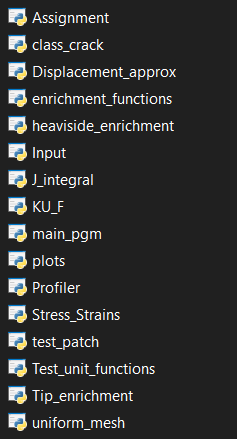
\includegraphics[scale =1]{ppp_files.PNG}
    \caption{Files necessary to run the program}
%    \label{fig:14}
    \centering
\end{figure}

\subsection{Libraries}
The list of inbuilt libraries and their versions used in the program is given below
\\
numpy: 1.18.5 \newline
scipy: 1.5.0 \newline
matplotlib: 3.2.2 \newline
shapely: 1.8.0 \newline

\subsection{Flow charts}
The below illustrations \autoref{fig:15} and \autoref{fig:16} give a basic overview on the program flow.
\begin{figure}[H]
    \centering
    \includegraphics[scale =0.4]{flowchart _1.drawio.png}
    \vspace{0.5cm}
    \caption{Flow chart for the selection of elements}
    \label{fig:15}
\end{figure}

\begin{figure}[H]
    \centering
    \includegraphics[width=9.5cm, scale =0.28]{J-integral.drawio.png}
    \caption{Flow chart calculate SIFs}
    \label{fig:16}
\end{figure}

\section{\large Testing and verification}
All the tests that have been carried out are discussed in detail in this section.
\subsection{\large Unit tests}
\subsubsection{Sanity check for Step function}
\textbf{Aim}: To check if the step function is producing proper outputs\newline
\textbf{Procedure}: 4 nodal coordinates, and crack coordinates are required to carryout the test see.~\autoref{fig:17}. The output will be 1,-1 or 0 based on the location of the nodes w.r.t the crack segment. The outputs act as the inputs in generating Heaviside B-matrix For the below shown figure, the expected outputs are listed below.
\\
{ \rule{\linewidth}{0.05cm}}
	{\scshape Function Body For Heaviside Step Function}\\
{ \rule{\linewidth}{0.05cm}}
{\fontfamily{qcr}\selectfont
\\
\textbf{def step{\_}function(A, cracks)\\
    Parameters\\
    A : point under query\\
    cracks : all the crack segment coordinates\\
    Returns: 1 or 0 or -1\\
    }}
\begin{figure}[h]
    \centering
    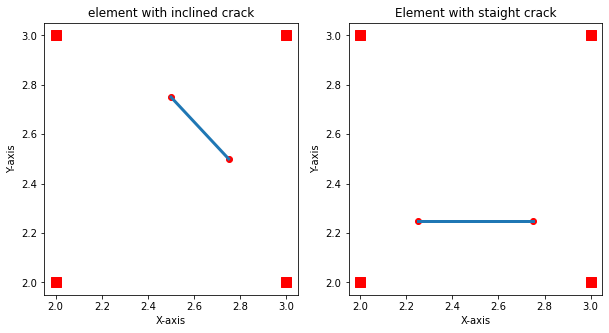
\includegraphics[width = 10cm, scale = 0.30]{step function.png}
    \caption{Crack segments inside an element \\Left: inclined crack, Right : straight crack }
    \label{fig:17}
    \centering
\end{figure}   

\hspace{-0.5cm}\textbf{Expected output-1}: For inclined crack, [-1,-1, 1,-1] \newline
\textbf{Expected output-2}: For straight crack, [-1,-1, 1, 1]\newline
\textbf{Result}:Test case passed
\\
{\rule{\linewidth}{0.02cm}}\\
command to run the test: {\fontfamily{qcr}\selectfont \testbf{py.test -v Test{\_}unit{\_}functions.py::test{\_}step{\_}function}}\\
command to check the output: {\fontfamily{qcr}\selectfont \testbf{python -c 'import Test{\_}unit{\_}functions;\\ Test{\_}unit{\_}functions.test{\_}step{\_}function()'}}\\
{ \rule{\linewidth}{0.02cm}}
\subsubsection{Sanity check for Heaviside B-matrix}
\textbf{Aim}: To check if Heaviside function is producing proper outputs as per the corresponding Heaviside function values \newline
\textbf{Procedure}: After generating a enriched shape function matrix of shape 2x4, these functions are called to generate individual B-matrices of size 3x2.
For the below enriched shape function matrix, a sample B-matrix is as expected.
\\
{\rule{\linewidth}{0.05cm}}
	{\scshape Function Body For Heaviside B-matrix Generation}\\
{\rule{\linewidth}{0.05cm}}
{\fontfamily{qcr}\selectfont
\\
\textbf{def heaviside{\_}function1(dN{\_}en, H1)\\
    The function generates a B-matrix for the "lower left" node w.r.t crack tip\\
    Parameters\\
    ----------\\
    dN{\_}en : differentiated shape function W.r.t x and y (2x4 shape)\\
    H1 : step function value for the "lower left" node\\
    Returns\\
    -------\\
    B{\_}enriched1 : Enriched B-matrix for lower left node\\
}}
\textbf{Input}: 
$$
    \pdv{[N]}{(x,y)} = \large \begin{bmatrix} 
    \dv{N_i} {x} \\[7pt]
    \dv{N_i} {y} \\
    \end{bmatrix} \large
    =
    \begin{bmatrix}
    1 & 1 & 1 & 1 \\
    1 & 1 & 1 & 1 \\
    \end{bmatrix}
    $$
\\                
\textbf{Expected output for node 1}:
$$
\left[\begin{array}{ll}
1 & 0 \\
0 & 1 \\
1 & 1
\end{array}\right]
$$
\textbf{Result}:Test case passed
\\
{\rule{\linewidth}{0.02cm}}\\
command to run the test: {\fontfamily{qcr}\selectfont \testbf{py.test -v Test{\_}unit{\_}functions.py::test{\_}heaviside{\_}functions}}\\
command to check the output: {\fontfamily{qcr}\selectfont \testbf{python -c 'import Test{\_}unit{\_}functions;\\ Test{\_}unit{\_}functions.test{\_}heaviside{\_}functions()'}}\\
{ \rule{\linewidth}{0.02cm}}

\vspace{-0.5cm}
\subsubsection{Sanity check for Connectivity matrix}
\textbf{Aim}: To check if the function is producing an identity matrix of size 8x8 for the particular input\newline
\textbf{Procedure}: For a given element number (list of 4 numbers), the function generates a connectivity matrix of size 8x8.
\\
{ \rule{\linewidth}{0.05cm}}
	{\scshape Function Body For Reshaping The Matrix}\\
{ \rule{\linewidth}{0.05cm}}
{\fontfamily{qcr}\selectfont
\\
\textbf{def connectivity{\_}matrix(EL, KL, length{\_}nodes, Hside, Tside)\\
    The function computes Assignment matrix for all the types of the elements\\
    Parameters\\
    EL : Element list [1,2,3,4]\\
    KL : List of stiffness matrices\\
    length{\_}nodes : Total nodes present in the geometry\\
    Hside : List of nodes that are heaviside enriched\\
    Tside : List of nodes that are tip enriched\\
    Returns\\
    -------\\
    K{\_}global : assembled stiffness matrix\\
    Total{\_}Normal{\_}DOFs : Total classical DOFs\\
    Total{\_}Dofs : Total Geometry DOFs\\
    Tside = sorted list of nodes that are tip enriched\\
    Hside = sorted list of nodes that are Heaviside enriched\\
    }}
\textbf{Input}: [0,1,3,2]
\newline                   
\textbf{Expected output}:
$$
 \begin{bmatrix}
1 & 0 & 0 & 0 & 0 & 0 & 0 & 0 \\
0 & 1 & 0 & 0 & 0 & 0 & 0 & 0 \\
0 & 0 & 1 & 0 & 0 & 0 & 0 & 0 \\
0 & 0 & 0 & 1 & 0 & 0 & 0 & 0 \\
0 & 0 & 0 & 0 & 1 & 0 & 0 & 0 \\
0 & 0 & 0 & 0 & 0 & 1 & 0 & 0 \\
0 & 0 & 0 & 0 & 0 & 0 & 1 & 0 \\
0 & 0 & 0 & 0 & 0 & 0 & 0 & 1 \\
\end{bmatrix}
$$
\textbf{Result}:Test case passed
\\
{\rule{\linewidth}{0.02cm}}\\
command to run the test: {\fontfamily{qcr}\selectfont \testbf{py.test -v Test{\_}unit{\_}functions.py::test{\_}connectivity{\_}matrix}}\\
command to check the output: {\fontfamily{qcr}\selectfont \testbf{python -c  'import Test{\_}unit{\_}functions;\\
Test{\_}unit{\_}functions.test{\_}connectivity{\_}matrix()}}\\
{\rule{\linewidth}{0.02cm}}

\subsubsection{Sanity check for addAtpos function}
\textbf{Aim}: To check if the function is producing a matrix of desired order \newline
\textbf{Procedure}: For a given matrix, the function changes the order of the matrix by adding extra zeros.\\
\\
{ \rule{\linewidth}{0.05cm}}
	{\scshape Function Body For Reshaping The Matrix}\\
{ \rule{\linewidth}{0.05cm}}
{\fontfamily{qcr}\selectfont
\\
\textbf{def addAtPos(dummy, matrix)\\
    This function is created to balance the size of the matrices. This function is called when the size of the matrix is not  40X40, the highest possible size for a matrix in the sample. The function adds two matrices of different sizes in place, offset by xy \newline 
    coordinates.\\
    Usage:\\
    ----------\\
    matrix: base matrix\\
    dummy: add this matrix to base matrix\\
    pos: tuple (x,y) containing the location where the matrix to be added\\
    Returns\\
    result : Matrix\\
    }}
\textbf{Input}: Input matrix shape 4x4
$$
 \begin{bmatrix}
0 & 1 & 2 & 3 \\
4 & 5 & 6 & 7 \\
8 & 9 & 10 & 11 \\
12 & 13 & 14 & 15 
\end{bmatrix}
$$
\textbf{Expected output}: Output size 5x5 
$$
 \begin{bmatrix}
0 & 1 & 2 & 3 & 0 \\
4 & 5 & 6 & 7 & 0 \\
8 & 9 & 10 & 11 & 0 \\
12 & 13 & 14 & 15 & 0 \\
0 & 0& 0& 0& 0&
\end{bmatrix}
$$
\textbf{Result}:Test case passed
\\
{\rule{\linewidth}{0.02cm}}\\
command to run the test: {\fontfamily{qcr}\selectfont \testbf{py.test -v Test{\_}unit{\_}functions.py::test{\_}addAtPos}}\\
command to check the output: {\fontfamily{qcr}\selectfont \testbf{python -c 'import Test{\_}unit{\_}functions; \\
Test{\_}unit{\_}functions.test{\_}addAtPos()'}}\\
{\rule{\linewidth}{0.02cm}}

\subsubsection{Sanity check for node filtering}
\textbf{Aim}: To check if the function is filtering the unwanted lists properly \newline
\textbf{Procedure}: For a given list of nodal coordinates, the function filters out the inner lists which are enriched.
\\
{ \rule{\linewidth}{0.05cm}}
	{\scshape Function Body For Node Filtering}\\
{ \rule{\linewidth}{0.05cm}}
{\fontfamily{qcr}\selectfont
\\
\textbf{def filtering(EN{\_}list, GL{\_}nodes)\\
    This function filters the nodes which do not require enrichment\\
    Parameters\\
    ----------\\
    EN{\_}list : List of nodes which has been enriched\\
    GL{\_}nodes : list containing all the nodes\\
    Returns\\
    -------\\
    result : Filtered nodes\\
    }}
\textbf{Input}: List of lists of nodal coordinates
\begin{center}
((2.0, 2.0), (3.0, 2.0), (3.0, 3.0), (2.0, 3.0))\\
((0.0, 2.0), (1.0, 2.0), (1.0, 3.0), (0.0, 3.0))\\
((1.0, 2.0), (2.0, 2.0), (2.0, 3.0), (1.0, 3.0))\\
((0.0, 0.0), (1.0, 0.0), (1.0, 1.0), (0.0, 1.0))\\
((1.0, 0.0), (2.0, 0.0), (2.0, 1.0), (1.0, 1.0))\\
((2.0, 0.0), (3.0, 0.0), (3.0, 1.0), (2.0, 1.0))\\
\textbf{((3.0, 0.0), (4.0, 0.0), (4.0, 1.0), (3.0, 1.0))}\\
\end{center}
\textbf{Enriched nodal list}:
\begin{center}
((3.0, 0.0), (4.0, 0.0), (4.0, 1.0), (3.0, 1.0))
\end{center}
\newline
\textbf{Expected output}: After filtering
\begin{center}
((2.0, 2.0), (3.0, 2.0), (3.0, 3.0), (2.0, 3.0))\\
((0.0, 2.0), (1.0, 2.0), (1.0, 3.0), (0.0, 3.0))\\
((1.0, 2.0), (2.0, 2.0), (2.0, 3.0), (1.0, 3.0))\\
((0.0, 0.0), (1.0, 0.0), (1.0, 1.0), (0.0, 1.0))\\
((1.0, 0.0), (2.0, 0.0), (2.0, 1.0), (1.0, 1.0))\\
((2.0, 0.0), (3.0, 0.0), (3.0, 1.0), (2.0, 1.0))\\
\end{center}
\\
\textbf{Result}: Test case passed
\\
{\rule{\linewidth}{0.02cm}}\\
command to run the test: {\fontfamily{qcr}\selectfont \testbf{py.test -v Test{\_}unit{\_}functions.py::test{\_}node{\_}filtering}}\\
command to check the output: {\fontfamily{qcr}\selectfont \testbf{python -c  'import Test{\_}unit{\_}functions; \\
Test{\_}unit{\_}functions.test{\_}node{\_}filtering()'}}\\
{\rule{\linewidth}{0.02cm}}
\subsubsection{Sanity check for element filtering}
\textbf{Aim}: To check if the function is filtering the unwanted lists properly \newline
\textbf{Procedure}: For a given list of element numbers, the function filters out the inner lists which are enriched.
{ \rule{\linewidth}{0.05cm}}
	{\scshape Function Body For Element Filtering}\\
{ \rule{\linewidth}{0.05cm}}
{\fontfamily{qcr}\selectfont
\\
\textbf{def E{\_}filter(EN{\_}list, GL{\_}elements)\\
    This function filters the elements which do not require enrichment\\
    Parameters\\
    ----------\\
    EN{\_}list : Enriched element list\\
    GL{\_}elements :  list containing all the elements\\
    Returns\\
    -------\\
    result : filtered elements\\
    }}\\
\textbf{Input}: List of lists of element numbers
\begin{center}
(14.0, 15.0, 21.0, 20.0), (12.0, 13.0, 19.0, 18.0)\\
(13.0, 14.0, 20.0, 19.0), (10.0, 11.0, 17.0, 16.0)\\
\textbf{(16.0, 17.0, 23.0, 22.0)},\textbf{(22.0, 23.0, 29.0, 28.0)} \\
\end{center}
\\
\textbf{Enriched element list}:
\begin{center}
((22.0, 23.0, 29.0, 28.0), (16.0, 17.0, 23.0, 22.0))
\end{center}
\\
\textbf{Expected output}: After removing the enriched element list
\begin{center}
(14.0, 15.0, 21.0, 20.0)\\
(12.0, 13.0, 19.0, 18.0)\\
(13.0, 14.0, 20.0, 19.0)\\
(10.0, 11.0, 17.0, 16.0)
\end{center}
\textbf{Result}: Test case passed
\\
{\rule{\linewidth}{0.02cm}}\\
Command to run the test: {\fontfamily{qcr}\selectfont py.test -v  Test{\_}unit{\_}functions.py::test{\_}E{\_}filter}\\
Command to check the output: {\fontfamily{qcr}\selectfont python -c ’import Test{\_}unit{\_}functions;\\
Test{\_}unit{\_}functions.test{\_}E{\_}filter()’}\\
{\rule{\linewidth}{0.02cm}}
\subsubsection{Sanity check for Gauss points generation}
\textbf{Aim}: To check if the function is generating the Gauss point coordinates properly  \newline
\textbf{Procedure}: For a given list of nodal coordinates, the function generates Gauss points at the calculated distance.
\\
{ \rule{\linewidth}{0.05cm}}
	{\scshape Function Body For Gauss Points Generation}\\
{ \rule{\linewidth}{0.05cm}}
{\fontfamily{qcr}\selectfont
\\
\textbf{def G{\_}points(SE{\_}ME)\\
    The function plots the Gauss points in the global coordinate system\\
    Parameters\\
    ----------\\
    SE{\_}ME : list of nodes to calculate the coordinates of new Gauss points\\
    Returns\\
    -------\\
    G : List of 4 Gauss points\\
    GPs : returns 1 Gauss point\\
    }}\\
\textbf{Input}: List of nodal coordinates
\begin{center}
((2.0, 2.0), (3.0, 2.0), (3.0, 3.0), (2.0, 3.0))\\
\end{center}
\hspace{-0.15cm}
\textbf{Expected coordinates}:
\begin{center}
((2.25, 2.25), (2.75, 2.25), (2.75, 2.75), (2.25, 2.75))
\end{center}
\textbf{Result}: Test case passed
\\
{\rule{\linewidth}{0.02cm}}\\
Command to run the test: {\fontfamily{qcr}\selectfont py.test -v Test{\_}unit{\_}functions.py::test{\_}Gausspoints}\\
Command to check the output: {\fontfamily{qcr}\selectfont python -c 'import Test{\_}unit{\_}functions;\\ Test{\_}unit{\_}functions.test{\_}Gausspoints()'}\\
{\rule{\linewidth}{0.02cm}}

\subsubsection{Sanity check for Asymptotic functions}
\textbf{Aim}: To check if the function is generating right values for the given r and $\theta$, $\alpha$ values\newline
\textbf{Procedure}: For a given list of nodal coordinates, the function generates Gauss points at the calculated distance.
\\
{ \rule{\linewidth}{0.05cm}}
	{\scshape Function Body For Asymptotic functions Generation}\\
{ \rule{\linewidth}{0.05cm}}
{\fontfamily{qcr}\selectfont
\\
\textbf{def asymptotic{\_}functions(r, theta, alpha)\\
    This function generates the necessary terms required for generating tip enriched \newline 
    B-matrix.\\
    Parameters\\
    ----------\\
    r : polar coordinate of the point under query, measured from the crack tip\\
    theta : angle of the point under query, measured from the crack tip (-pi to +pi)\\
    alpha : angle made by crack w.r.t global x-axis\\
    Returns\\
    -------\\
    F1 : asymptotic{\_}function1\\
    F2 : asymptotic{\_}function2\\
    F3 : asymptotic{\_}function3\\
    F4 : asymptotic{\_}function4\\
    dF : Differentiation of the enrichment functions associated with Shape functions\\
}}
\textbf{Input}: $r=0.25$ and $\theta = 0.15935$, $\alpha=0$\\ 
\textbf{Expected output}:
\begin{center}
( 0.98916395, -0.14681514, -0.14681514, -0.98916395, -0.26253043, -1.85407775,
 -0.12425015, -0.5561607)
\end{center}
\\
\textbf{Result}: Test case passed
\\
{\rule{\linewidth}{0.02cm}}\\
command to run the test: {\fontfamily{qcr}\selectfont py.test -v Test{\_}unit{\_}functions.py::test{\_}asymptotic{\_}functions}\\
command to check the output: {\fontfamily{qcr}\selectfont python -c 'import Test{\_}unit{\_}functions;\\
Test{\_}unit{\_}functions.test{\_}asymptotic{\_}functions()}\\
{\rule{\linewidth}{0.02cm}}

\subsubsection{Sanity check for Tip enriched B-matrix}
\textbf{Aim}: To check if the function is generating proper B-matrix values for the given input\newline
\textbf{Procedure}: For a given list of nodal coordinates, shape functions, Jacobian matrix, differentiated shape functions, the function generates a B-matrix of shape 8x8.
\\
{ \rule{\linewidth}{0.05cm}}
	{\scshape Function Body For Tip Enriched B-matrix Generation}\\
{ \rule{\linewidth}{0.05cm}}
{\fontfamily{qcr}\selectfont
\\
\textbf{def tip{\_}enrichment{\_}func{\_}N1(F1, F2, F3, F4, dN, dF, N)\\
    The function generates a B-matrix for the "Lower left" node w.r.t the\\ corresponding element\\
    Parameters\\
    ----------\\
    F1 : asymptotic{\_}function1\\
    F2 : asymptotic{\_}function2\\
    F3 : asymptotic{\_}function3\\
    F4 : asymptotic{\_}function4\\
    dF : Differentiation of the enrichment functions associated with Shape functions\\
    dN : Differentiation of Shape functions w.r.t x and y (2x4 shape)\\
    N : Shape function values\\
    Returns\\
    -------\\
    B{\_}tip1 : B-matrix for "Lower left" node (3x8 shape)\\
}}
\textbf{Input}:
\begin{center}
((2.0, 2.0), (3.0, 2.0), (3.0, 3.0), (2.0, 3.0))\\
Shape functions: N1, N2, N3, N4\\
Asymptotic function values: F1, F2, F3, F4

\end{center}
\textbf{Expected output}:
\begin{center}
((0.14869175,  0, 0.00895635,  0, 0.0186328, 0. -0.00104311,  0)\newline
 (0, 0.09796097,  0,-0.02866144,  0,-0.05244283, 0, -0.02033145)\newline
 (0.09796097, 0.14869175, -0.02866144, 0.00895635, -0.05244283, 0.0186328, -0.02033145, -0.00104311))
\end{center}
\\
\textbf{Result}: Test case passed\\
\newline
{\rule{\linewidth}{0.02cm}}\\
Command to run the test: {\fontfamily{qcr}\selectfont py.test -v Test{\_}unit{\_}functions.py::test{\_}tip{\_}enrichment{\_}func{\_}N1}\\
Command to check the output: {\fontfamily{qcr}\selectfont python -c 'import Test{\_}unit{\_}functions;\\
Test{\_}unit{\_}functions.test{\_}tip{\_}enrichment{\_}func{\_}N1()'}\\
{\rule{\linewidth}{0.02cm}}

\subsubsection{Sanity check for Uniform mesh}
\textbf{Aim}: To check if the function is producing proper nodal coordinates and element numbering in CCW direction\newline
{ \rule{\linewidth}{0.05cm}}
	{\scshape Function Body For Uniform Mesh Generation}\\
{ \rule{\linewidth}{0.05cm}}
{\fontfamily{qcr}\selectfont
\\
\textbf{def uniform{\_}mesh(A,B,x)\\
    This function computes all the prerequisites for the nodes and elements generations\\
    Parameters\\
    -----------\\
    A : length along x{\_}axis\\
    B : length along y{\_}axis\\
    x : number of elements per row\\
    Returns\\
    NL : list of nodes\\
    EL : list of elements\\
    }}
\textbf{Inputs}: length of the geometry along x and y axes A = 1unit, B = 1unit.\\
Divisions along x and y axis, x = 1\\
\textbf{Expected output-1}: Nodal coordinates
\begin{center}
((0, 0),(1, 0),(0, 1),(1, 1))
\end{center}
\textbf{Expected output-2}: Element numbering
\begin{center}
(1,2,4,3)
\end{center}
\textbf{Result}: Test case passed
\\
{\rule{\linewidth}{0.02cm}}\\
command to run the test: {\fontfamily{qcr}\selectfont py.test -v Test{\_}unit{\_}functions.py::test{\_}uniform{\_}mesh}\\
command to check the output: {\fontfamily{qcr}\selectfont python -c  'import Test{\_}unit{\_}functions; \\
Test{\_}unit{\_}functions.test{\_}uniform{\_}mesh()'}\\
{\rule{\linewidth}{0.02cm}}

\subsubsection{Sanity check for Strain matrix generator}
\textbf{Aim}: To check if the function is producing proper strains using small strain theory see.~\autoref{eq:110}. The equation is given below\newline
{ \rule{\linewidth}{0.05cm}}
	{\scshape Function Body For Strain Matrix Generation}\\
{ \rule{\linewidth}{0.05cm}}
{\fontfamily{qcr}\selectfont
\\
\textbf{def Kinematics(grad{\_}disps):\\
    Applying small strain theory, the function computes auxiliary strains from the\\ auxiliary displacements\\
    $\epsilon_{ij}$ = 0.5*(Ui,j + Uj,i)\\
    Parameters\\
    ----------\\
    grad{\_}disps : Auxiliary displacements\\
    Returns: Auxiliary strains\\
    }}
\begin{align}\label{eq:110}\hspace{4.5cm}
\epsilon_{ij}  =  0.5 * \begin{bmatrix}
U_{i,i} + U_{i,i} & U_{i,j} + U_{j,i}\\
U_{j,i} + U_{i,j} & U_{j,j} + U_{j,j}\\
\end{bmatrix}
\end{align}
\\
\textbf{Inputs}:Displacement matrix of shape 2x2
$$
 \begin{bmatrix}
1 & 1\\
2 & 2\\
\end{bmatrix}
$$
\\
\textbf{Expected output-1}: Strains computed considering small strain theory
$$
 \begin{bmatrix}
1 & 1.5\\
1.5 & 2\\
\end{bmatrix}
$$
\textbf{Result}: Test case passed
\\
{\rule{\linewidth}{0.02cm}}\\
command to run the test: {\fontfamily{qcr}\selectfont py.test -v Test{\_}unit{\_}functions.py::test{\_}kinematics}\\
command to check the output: {\fontfamily{qcr}\selectfont python -c 'import Test{\_}unit{\_}functions;\\
Test{\_}unit{\_}functions.test{\_}kinematics()'}\\
{\rule{\linewidth}{0.02cm}}

\subsubsection{Sanity check for point inside the circle}
\textbf{Aim}: To check if the nodal coordinates lie inside or outside the prescribed circle\newline
{ \rule{\linewidth}{0.05cm}}
	{\scshape Function Body To Check of Point Lie Outside The Domain}\\
{ \rule{\linewidth}{0.05cm}}
{\fontfamily{qcr}\selectfont
\textbf{def inside{\_}circ(c{\_}2, length{\_}element{\_}x, length{\_}element{\_}y, P, scale)\\
    The function checks if any of the nodes is outside the domain under consideration. If yes, it will return True, False otherwise\\
    Parameters\\
    ----------\\
    c{\_}2 : right crack tip\\
    length{\_}element{\_}x : length of the element along x-direction in "meters"\\
    length{\_}element{\_}y : length of the element along y-direction in "meters"\\
    P : point under query (nodes)\\
    scale : scaling factor of the domain used for interaction integral\\
    Returns\\
    -------\\
    nodal value (q) 1 or 0 based on the condition\\
    }}
\textbf{Inputs}: Crack tip = (0.5,0.5)\\ 
length of element along x and y = 1\\
Nodal coordinates = [2,2]\\
scale of the circle = 1.5\\
\textbf{Expected output}: False (point lie outside the circle for the given inputs)\\
\textbf{Result}: Test case passed
\\
{\rule{\linewidth}{0.02cm}}\\
command to run the test: {\fontfamily{qcr}\selectfont py.test -v Test{\_}unit{\_}functions.py::test{\_}inside{\_}circ}\\
command to check the output: {\fontfamily{qcr}\selectfont python -c 'import Test{\_}unit{\_}functions;\\
Test{\_}unit{\_}functions.test{\_}inside{\_}circ()'}\\
{\rule{\linewidth}{0.02cm}}

\subsubsection{Sanity check matrix transformation}
\textbf{Aim}: To check if the function is able to properly transform the matrix from global system to local crack tip coordinate system see.~\autoref{eq:111}\newline
{ \rule{\linewidth}{0.05cm}}
	{\scshape Function Body For Matrix Transformation}\\
{ \rule{\linewidth}{0.05cm}}
{\fontfamily{qcr}\selectfont
\textbf{def Global{\_}to{\_}local{\_}CT(S, CTCS)\\
    CTCS = Rotation Matrix\\
    Parameters\\
    ----------\\
    S : stresses in global co-ordinate system\\
    CTCS : crack tip coordinate system\\
    Returns\\
    -------\\
    Stresses in local crack coordinate system\\
    }}
\textbf{Inputs}: crack angle w.r.t x-axis, $\alpha = 90^o$\\ 
random matrix = [1,2,3]\\
Rotation matrix = 
\begin{align}\label{eq:111}\hspace{6.5cm}
\begin{bmatrix}
\cos\alpha & \sin\alpha\\
-\sin\alpha & \cos\alpha\\
\end{bmatrix}
\end{align}
\textbf{Expected output}: For the current input, the corresponding output is as expected  
 $$ 
\begin{bmatrix}
-0.60422787 & -2.19595653\\
-2.19595653 & 3.60422787\\
\end{bmatrix}
$$
\textbf{Result}: Test case passed
\\
{\rule{\linewidth}{0.02cm}}\\
command to run the test: {\fontfamily{qcr}\selectfont py.test -v Test{\_}unit{\_}functions.py::test{\_}Global{\_}to{\_}local{\_}CT}\\
command to check the output: {\fontfamily{qcr}\selectfont python -c  'import Test{\_}unit{\_}functions;\\
Test{\_}unit{\_}functions.test{\_}Global{\_}to{\_}local{\_}CT()'}\\
{\rule{\linewidth}{0.02cm}}

\subsection{\large Patch tests}
\subsubsection{Rigid body translation test}
\textbf{Aim}: To check if the inner node has the same displacement as the outer nodes.\newline
\textbf{Procedure}: In this case, we consider a 2x2 elements and prescribe a displacements on the outer nodes of the geometry see.~\autoref{fig:18} and then we check the displacements of the inner node.\newline
\textbf{Example}: A geometry consisting of 2x2 elements with 9 nodes see.~\autoref{fig:18}, node number 5 is considered as the inner node. It shares its position with all the 4 elements. Here, we prescribe displacements on the 4 corner nodes of the geometry. One should make sure that the geometry is in equilibrium.
\begin{figure}[h]
    \centering
    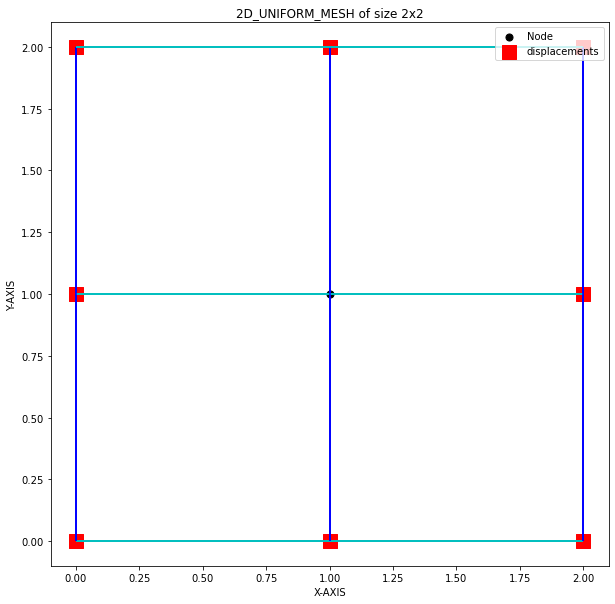
\includegraphics[scale=0.40]{2x2 disp.png}
    \caption{Sample under translation patch test\\ Red squares:             Prescribed displacements}
    \label{fig:18}
\end{figure}
\\
\textbf{Expected output}: If a displacement of 0.5mm both in x and y directions is prescribed, the inner node should displace at about the same (0.5mm) as the corner nodes. \newline
\textbf{Result}: Test case passed\\
\\
{\rule{\linewidth}{0.02cm}}\\
Command to run the test: {\fontfamily{qcr}\selectfont py.test -v test{\_}patch.py::test{\_}displacement{\_}2x2}\\
Command to check the output: {\fontfamily{qcr}\selectfont python -c 'import test{\_}patch;\\
test{\_}patch.test{\_}displacement{\_}2x2()'}\\
{\rule{\linewidth}{0.02cm}}

\subsubsection{Linear Elastic Material Response test}
This test checks if the selected element is a Linear elastic or not. The easiest method is to implement Newton's method \cite{taylor2014feap}.\newline
\textbf{Aim}: To check if the material response in linear elastic in nature by implementing Newton's method.\newline
\textbf{Procedure}: Here, 4 elements are considered for the test which are skewed towards the right. All the nodes in the extreme right are prescribed with traction boundary conditions and the nodes that are in the extreme left are prescribed with essential boundary conditions.\newline
\textbf{Example}: In the below figure \autoref{fig:19}, the bottom right node is prescribed with 2.5N, the top right node is prescribed with 2.5N, and the middle node is prescribed with 5N forces. Both the degrees of freedom are arrested for the  bottom right node. $U_x$ is arrested for the other 2 nodes. The basic idea of  the implementation is given below. 

\begin{figure}[h]
    \centering
    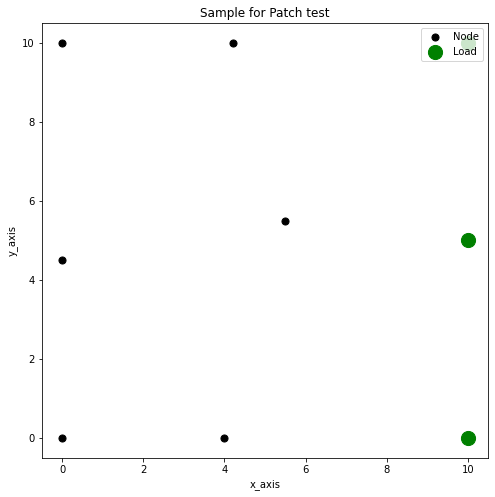
\includegraphics[scale =0.55]{Newton's.png}
    \caption{Sample under patch test\\ Green circles: Prescribed force}
    \label{fig:19}
\end{figure}

\hspace{-0.5cm}Consider the equilibrium equation see.~\autoref{eq:112}
\begin{align}\label{eq:112}\hspace{6.5cm}
\mathbf{R}(\mathbf{u})=\mathbf{F}-\mathbf{P}(\mathbf{u})
\end{align}
wherein $\mathbf{F}$ is the vector of applied nodal forces, $u$ is the vector of nodal displacements, and for a static linear elastic problem $\mathrm{P}$ is defined as see.~\autoref{eq:113}
\begin{align}\label{eq:113}\hspace{6.5cm}
\mathbf{P}=\mathbf{Ku}
\end{align}
in which $\mathbf{K}$ is the global stiffness matrix and $u$ is the initial displacement vector. A solution for the see.~\autoref{eq:112} is defined by requiring the residuals $\mathbf{R}$ to be zero. 

For the first iteration prescribe displacements as zero and calculate vector P and using the P vector, calculate residuals R using the see.~\autoref{eq:112}. With the new residuals compute a new displacement vector and add the new displacement vector to the older vector see.~\autoref{eq:114} then evaluate the above equation but now the residuals will be a zero vector.

\begin{align}\label{eq:114}\hspace{6.5cm}
\mathbf{u} \leftarrow \mathbf{u}+\Delta \mathbf{u}
\end{align}
\textbf{Expected output} : Convergence after one iteration\newline 
\textbf{Result}: Test case passed.\\
{\rule{\linewidth}{0.02cm}}\\
Command to run the test: {\fontfamily{qcr}\selectfont py.test -v test{\_}patch.py::test{\_}LE{\_}patch}\\
Command to check the output: {\fontfamily{qcr}\selectfont python -c 'import test{\_}patch;\\ test{\_}patch.test{\_}LE{\_}patch()'}\\
{\rule{\linewidth}{0.02cm}}

\subsubsection{Sanity check for Isotropic material property}
\textbf{Aim}: To check if the element is producing same stresses and strains at all the 4 Gauss points\cite{taylor2014feap}.\\
\textbf{Procedure}: Here, a single element is considered for the test see.~\autoref{fig:20}. The element is at equilibrium position under tensile load applied in Newtons. the equilibrium equation $\mathbf{Ku} = \mathbf{f}$, is solved to get the displacements and using these displacements, the stresses and strains are calculated at 4 Gauss points. The stresses and strains that are obtained must have same values at all the Gauss points. In the below figure stresses and strains have been computed at the red points.
\begin{figure}[h]
    \centering
    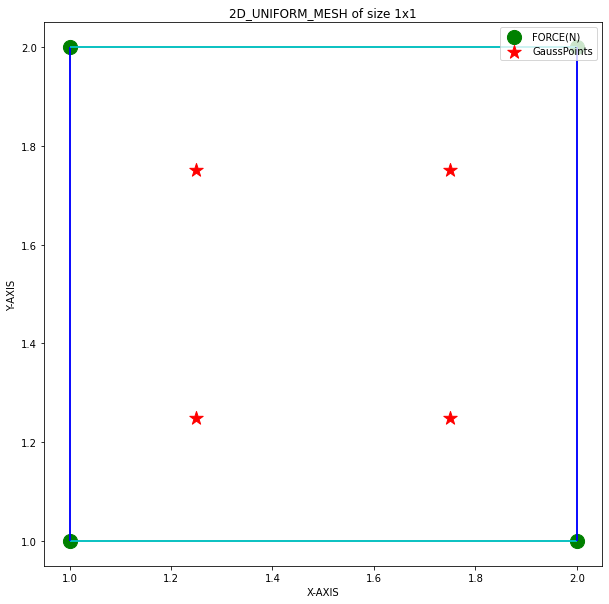
\includegraphics[scale = 0.5]{1x1 stress strain.png}
    \caption{{Stresses and strains for 1 element at 4 Gauss points}}
    \label{fig:20}
\end{figure}

\hspace{-0.5cm}\textbf{Expected output}: Same stresses and strains values at all the 4 Gauss points\newline
\textbf{Result}: Test case passed.
\\
{\rule{\linewidth}{0.02cm}}\\
Command to run the test: {\fontfamily{qcr}\selectfont py.test -v  test{\_}patch.py::test{\_}isotropic{\_}material{\_}prop}\\
Command to check the output: {\fontfamily{qcr}\selectfont python -c 'import test{\_}patch;\\
test{\_}patch.test{\_}isotropic{\_}material{\_}prop()'}\\
{\rule{\linewidth}{0.02cm}}

\subsubsection{Sanity check for Shape functions}
\textbf{Aim}: To check the properties of the shape functions\cite{pandey2019new}.\newline
\textbf{Procedure}: Here, for a 2d full integration scheme, 4 shape functions are taken into account. Initially, the summation of the shape functions are checked for one random Gauss point (Ex: $\frac{1}{\sqrt3}, \frac{1}{\sqrt3}$) and it should be 1 and the summation of the differentiated shape functions should be 0\newline  
\textbf{Expected output-1}: $$\sum_{i=1}^{4} N_i= 1$$
\textbf{Expected output-2}: $$\sum_{i=1}^{4} \pdv{N_i}{x}= 0 \hspace{1cm} \sum_{i=1}^{4} \pdv{N_i}{y}= 0$$
\textbf{Result}: Test case passed.

\subsubsection{Sanity check for Jacobian matrix}
\textbf{Aim}: To check if the Jacobian matrix obtained, is volume conserving or not irrespective of the rotation angle\cite{taylor2014feap}.\\
\textbf{Procedure}: For a given element coordinate system and Gauss points, a Jacobian matrix and its determinant is computed computed. Using Euler angles, the Jacobian matrix is rotated and then the determinant is computed.\newline 
\textbf{Expected output}: The determinant values before and after the rotation should remain same. This proves that Jacobian matrix is volume conserving. \newline
\textbf{Result}: Test case passed.
\\
{\rule{\linewidth}{0.02cm}}\\
Command to run the test: {\fontfamily{qcr}\selectfont py.test -v test{\_}patch.py::test{\_}Jacobian}\\
Command to check the output: {\fontfamily{qcr}\selectfont python -c 'import test{\_}patch;\\ test{\_}patch.test{\_}Jacobian()'}\\
{\rule{\linewidth}{0.02cm}}

\subsubsection{Sanity check for Rigid body motions}
\textbf{Aim}: To check if the global stiffness matrix is producing prescribed zeros for rotation and translation motion for the constrained and unconstrained structures. \cite{taylor2014feap}.\\
\textbf{Procedure}: For a given structure (1x1 element), global stiffness matrix is computed and then Eigenvalues are computed. If the 2D structure is unconstrained, then the number of zero Eigenvalues should be 3 (2-rotation, 1-translation). If one of the corners of the structure is constrained, then the number of zero Eigenvalues should be 0. \newline 
\textbf{Expected output}:Unconstrained structure=3 \newline
constrained structure = 0\\
\textbf{Result}: Test case passed.
\\
{\rule{\linewidth}{0.02cm}}\\
Command to run the test: {\fontfamily{qcr}\selectfont py.test -v test{\_}patch.py::test{\_}Rigid{\_}body{\_}motions}\\
{\rule{\linewidth}{0.02cm}}

\subsubsection{Sanity check for Rigid body rotation}
\textbf{Aim}: After performing the transformation, global stiffness matrix should be able to represent rigid body rotation \cite{taylor2014feap}.\\
\textbf{Procedure}: For a given structure (2x2 elements), all the nodes are rotated using the rotation matrix leading to the new positions. Now, the external nodes are rotated using transformation matrix. The new positions of the nodes acts as an input to the displacement vector. It should be mentioned here that the rotation is done w,r,t to the center node therefor, the displacement values of the center node is [0,0]. Using the available displacement and global stiffness matrix, the displacements of the inner node is calculated and compared with the initially rotated nodes.\newline 
\textbf{Expected output}:Inner node should have the displacement value of the initially rotated nodes\newline
\textbf{Result}: Test case passed.
\\
{\rule{\linewidth}{0.02cm}}\\
Command to run the test: {\fontfamily{qcr}\selectfont py.test -v test{\_}patch.py::test{\_}Rigid{\_}body{\_}rotation}\\
{\rule{\linewidth}{0.02cm}}
\\

\newpage
\section{\Large{Time Analysis}}
The first 3 lines of the log file has been used to create the time analysis section.
The first line gives the information on the name of the function. Second line gives the information on date, time and data (file name.prof). Third line indicates the number of function calls and time consumed by the CPU in seconds.

==========test{\_}uniform{\_}mesh==========\\
Fri Mar 25 07:51:34 2022 \tab[1cm] F1.prof \\
657 function calls (640 primitive calls) in 0.002 seconds\\

==========test{\_}kinematics==========\\
Fri Mar 25 07:51:34 2022 \tab[1cm]    F2.prof\\
1118 function calls (1089 primitive calls) in 0.004 seconds\\

==========test{\_}Global{\_}to{\_}local{\_}CT==========\\
Fri Mar 25 07:51:34 2022 \tab[1cm] F3.prof\\
1583 function calls (1542 primitive calls) in 0.005 seconds\\

==========test{\_}inside{\_}circ==========\\
Fri Mar 25 07:51:34 2022 \tab[1cm]   F4.prof\\
1640 function calls (1599 primitive calls) in 0.006 seconds\\

==========test{\_}step{\_}function==========\\
Fri Mar 25 07:51:35 2022 \tab[1cm]   F5.prof\\
357435 function calls (350183 primitive calls) in 0.702 seconds\\

==========test{\_}heaviside{\_}functions==========\\
Fri Mar 25 07:51:35 2022 \tab[1cm]  F6.prof\\
357826 function calls (350556 primitive calls) in 0.703 seconds\\
 
==========test{\_}addAtPos==========\\
Fri Mar 25 07:51:35 2022 \tab[1cm]   F7.prof\\
358804 function calls (351474 primitive calls) in 0.704 seconds\\

==========test{\_}connectivity{\_}matrix==========\\
Fri Mar 25 07:51:35 2022 \tab[1cm]   F8.prof\\
361449 function calls (353975 primitive calls) in 0.707 seconds\\

==========test{\_}node{\_}filtering==========\\
Fri Mar 25 07:51:35 2022 \tab[1cm]   F9.prof\\
361592 function calls (354118 primitive calls) in 0.707 seconds\\

==========test{\_}asymptotic{\_}functions==========\\
Fri Mar 25 07:51:35 2022 \tab[1cm]    F10.prof\\
362160 function calls (354670 primitive calls) in 0.709 seconds\\

==========test{\_}Gausspoints==========\\
Fri Mar 25 07:51:35 2022 \tab[1cm]   F11.prof\\
362791 function calls (355293 primitive calls) in 0.710 seconds\\

==========test{\_}tip{\_}enrichment{\_}func{\_}N1==========\\
Fri Mar 25 07:51:35 2022 \tab[1cm]   F12.prof\\
363995 function calls (356443 primitive calls) in 0.713 seconds\\

==========test{\_}E{\_}filter==========\\
Fri Mar 25 07:51:35 2022 \tab[1cm]    F13.prof\\
364112 function calls (356560 primitive calls) in 0.713 seconds\\

==========test{\_}LE{\_}patch==========\\
Fri Mar 25 07:51:35 2022 \tab[1cm]    F14.prof\\
440101 function calls (432078 primitive calls) in 6.792 seconds\\

==========test{\_}displacement{\_}2x2==========\\
Fri Mar 25 07:51:35 2022 \tab[1cm]   F15.prof\\
365116 function calls (357554 primitive calls) in 0.717 seconds\\

==========test{\_}isotropic{\_}material{\_}prop==========\\
Fri Mar 25 07:51:35 2022 \tab[1cm]    F16.prof\\
366298 function calls (358724 primitive calls) in 0.722 seconds\\

==========test{\_}Jacobian==========\\
Fri Mar 25 07:51:35 2022 \tab[1cm]   F17.prof\\
368182 function calls (360552 primitive calls) in 0.727 seconds\\

==========MainFunction==========\\
Fri Mar 25 20:25:37 2022 \tab[1cm]   F18.prof\\
2519091 function calls (2494063 primitive calls) in 24.391 seconds

\\
==========test{\_}Rigid{\_}body{\_}motion==========\\
Fri Mar 25 07:51:45 2022 \tab[1cm]   F19.prof\\
1892899 function calls (1856279 primitive calls) in 10.609 seconds\\

==========test{\_}Rigid{\_}body{\_}rotation==========\\
Fri Mar 25 07:51:45 2022 \tab[1cm]  F20.prof\\
1893919 function calls (1857289 primitive calls) in 10.612 seconds\\

\newpage
The below pie chart \autoref{fig:21} gives you an idea of the time elapsed by 
each function.
\\

\begin{figure}[h]
    \centering
    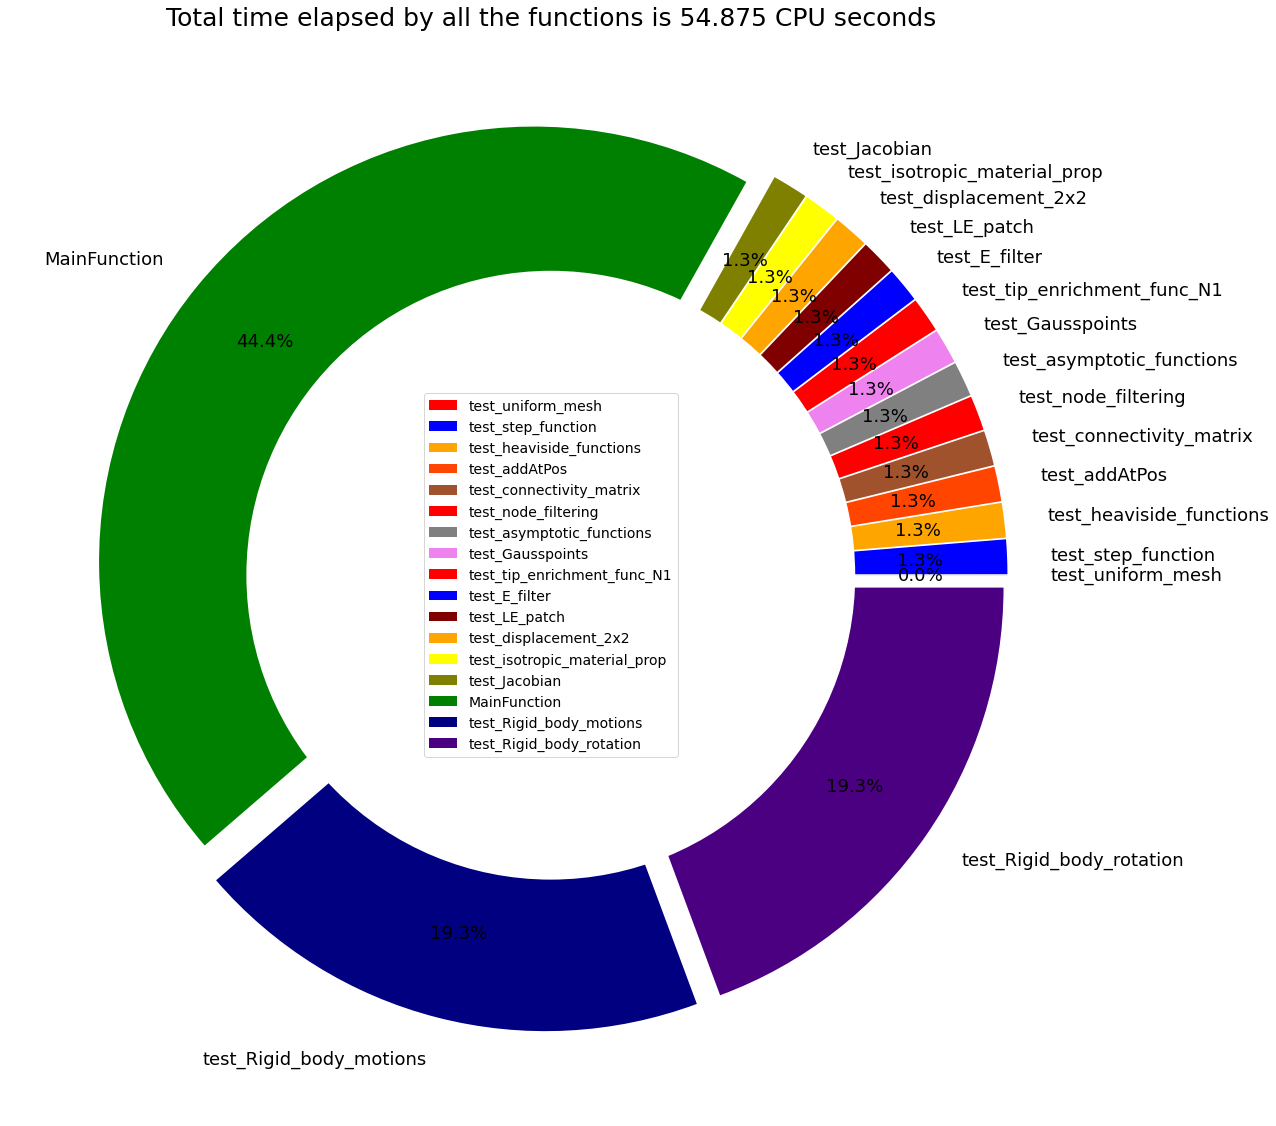
\includegraphics[scale = 0.35]{PIE.png}
    \caption{Time Analysis Pie Chart}
    \label{fig:21}
\end{figure}

\newpage
\bibliographystyle{plain}
\bibliography{ref}
\end{document}


